\chapter{Fourier-Theorie f"ur die Kugeloberfl"ache\label{chapter:kugel}}
\lhead{Fourier f"ur die Kugeloberfl"ache}
\begin{refsection}
\chapterauthor{Thomas Gujer und Christoph Schmitz-Dr"ager}

\section{Einleitung}
\rhead{Einleitung}

In diesem Kapitel m"ochten wir veranschaulichen, dass die Effekte welche man bei der klassischen Fourier-Theorie beobachten kann, auch bei der Fourier-Theorie auf der Kugeloberfl"ache zu sehen sind. Zur Visualisierung vergleichen wir jeweils ein Rechtecksignal mit dem Analogon auf der Kugeloberfl"ache.
 
\section{Kugelaufbau}
\rhead{Kugelaufbau}

\begin{figure}%Bild Koordinaten der Kugel
\centering
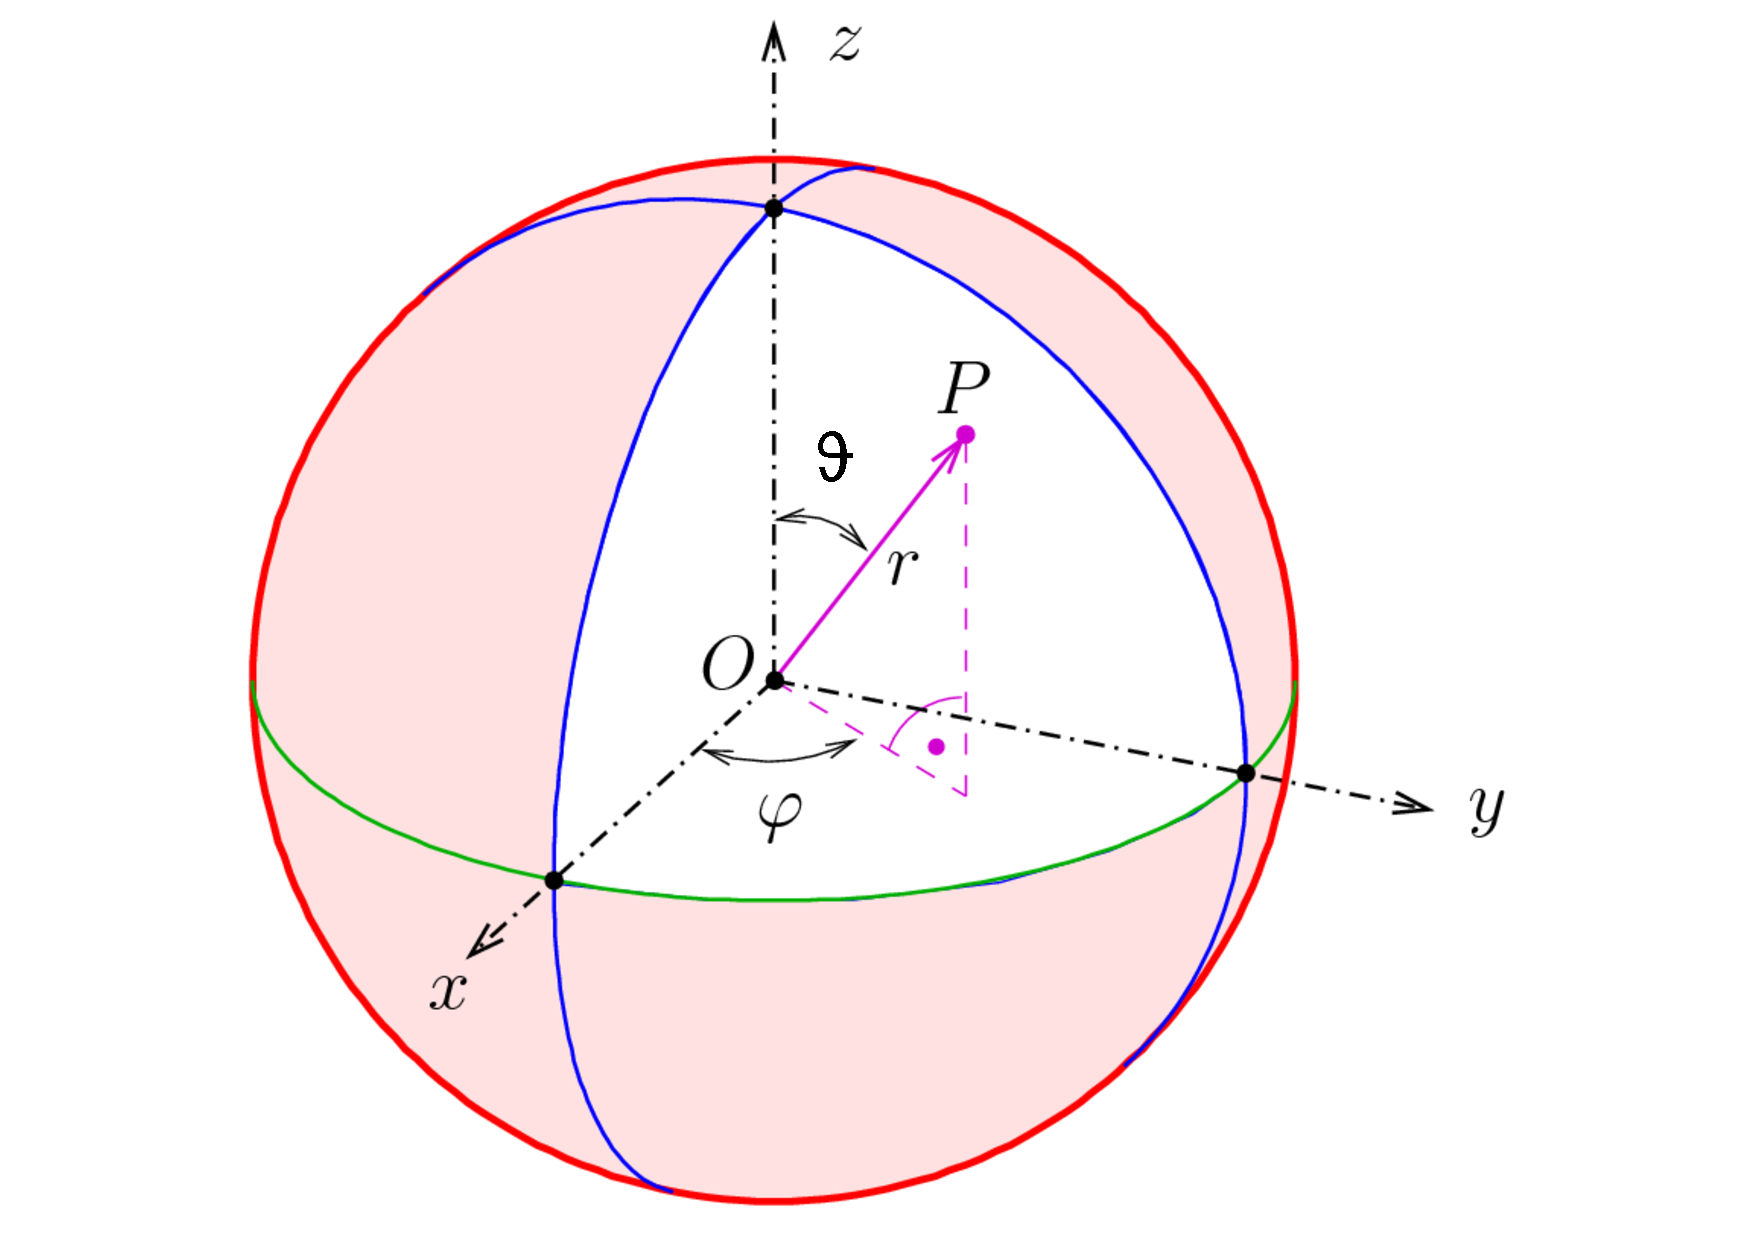
\includegraphics[width=0.7\textwidth]{kugel/Kugelkoord.pdf}
\caption{Koordinaten der Kugel
\label{skript:Koordinaten der Kugel}}
\end{figure}

In der Abbildung \ref{skript:Koordinaten der Kugel} 
ist zu sehen wie ein Punkt auf der Kugeloberfl"ache im Polar-Koordinaten definiert ist. Zum umrechnen ins kartesische Koordinatensystem werden folgende Formeln ben"otigt:
\begin{align*}
x& = r \cdot \sin\vartheta \cdot \cos\varphi 
\\
y& = r \cdot \sin\vartheta \cdot \sin\vartheta
\\
z& = r \cdot \cos\vartheta 
\end{align*}
 
 
\section{Aufbau der Funktion}
\rhead{Aufbau der Funktion}

\begin{figure}%Funktion auf Rechteckoberfläche 
\centering
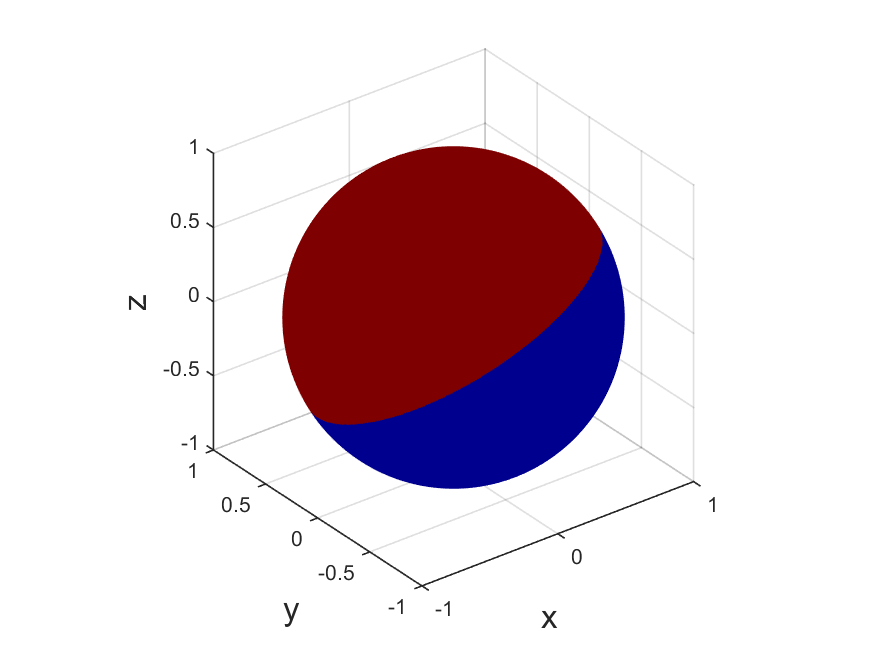
\includegraphics[width=0.7\textwidth]{kugel/Funktion.pdf}
\caption{Funktion auf Kugeloberfl"ache
\label{skript:Funktion auf Kugeloberfl"ache}}
\end{figure}

Es wird mit einer Funktion gearbeitet, welche 3 Variablen $f(x,y,z)$ bzw. $f(r,\vartheta,\varphi$) und einen Funktionswert besitzt. Der Radius ist in unserem Fall konstant = 1 das wir uns nur auf die Kugeloberfl"ache beziehen. Das Ziel ist, auf der Kugeloberfl"ache einem kreisf"ormigen Abschnitt den Wert 1 und dem Rest der Kugeloberfl"ache den Wert 0 zuzuweisen. Geometrisch (in der 3-dimensionalen Betrachtung) "andert sich die Kugel nicht. Der Funktionswert kann nur noch mit Farben dargestellt werden. Es ist dieselbe Darstellung, welche z.B. auch f"ur die Temperatur auf der Erdoberfl"ache verwendet wird. In diesem Fall sollte man die Form der Erde auch nicht beeinflussen um die Temperatur darzustellen. Deshalb verwendet man einen Farbschl"ussel f"ur die Darstellung der verschiedenen Temperaturen.\\

Die Funktion in diesem Kapitel wurde folgendermassen definiert:
\begin{enumerate}

\item Definition eines Vektors mit dem Startpunkt im Zentrum der Kugel und dem Endpunkt auf der Kugeloberfl"ache:

$$
\vec{c} = 
\begin{pmatrix}
{r \cdot \sin\vartheta \cdot \cos\varphi}\\
{r \cdot \sin\vartheta \cdot \sin\vartheta}\\
{r \cdot \cos\vartheta}
\end{pmatrix}
\text{mit r = 1 folgt}
\begin{pmatrix}
{\sin\vartheta \cdot \cos\varphi}\\
{\sin\vartheta \cdot \sin\vartheta}\\
{\cos\vartheta}
\end{pmatrix}
$$

\item	Des Weiteren wird ein Vektor definiert, welcher den Startpunkt im Zentrum der Kugel und den Endpunkt auf der Kugeloberfl"ache hat. Im Gegensatz zum $\vec{c}$ wo die Winkel $\vartheta$ und $\varphi$ eindeutig definiert sind besitzt der $\vec{r}$ ein variables $\vartheta$ von 0 bis $\pi$ und ein variables $\pi$ von $-\pi$ bis $\pi$: 

$$
\vec{r} = 
\begin{pmatrix}
{r \cdot \sin\vartheta \cdot \cos\varphi}\\
{r \cdot \sin\vartheta \cdot \sin\vartheta}\\
{r \cdot \cos\vartheta}
\end{pmatrix}
\text{mit r = 1 folgt}
\begin{pmatrix}
{\sin\vartheta \cdot \cos\varphi}\\
{\sin\vartheta \cdot \sin\vartheta}\\
{\cos\vartheta}
\end{pmatrix}
$$

\item
\[
f(x,y,z) =\begin{cases}
1& \qquad \text{wenn $\vec c\cdot\vec r$ $\ge$ 0 (Beispiel Halbkugel)}\\
0& \qquad \text{sonst}
\end{cases}
\]
\end{enumerate}

\section{Kugelfl"achenfunktionen}
\rhead{Kugelfl"achenfunktionen}

Kugelfl"achenfunktionen sind die Analoga zu den Sinus- und Kosinus-Funktionen bei der klassischen Fourier-Theorie. Mittels dieser Kugelfl"achenfunktionen $Y_{lm}$ und $Z_{lm}$ bildet man ein orthogonales System von Funktionen. Die Kugelfl"achenfunktionen sind wie folgt definiert:
\begin{align*}
Y_{lm}& = P_{lm} \cdot \cos(m \cdot \varphi)
\\
Z_{lm}& = P_{lm} \cdot \sin(m \cdot \varphi)
\end{align*}

Wobei es sich bei $P_{lm}$ um das in Kapitel (\ref{skript:legendreansatz}) hergeleitete Legendre-Polynom handelt. Wie in Abbildung \ref{skript:Bild 0} illustriert sieht man die verschiedenen Kugelfl"achenfunktionen vom Grad $l = 5$.

\begin{figure}% Bilder 0-2 Y_lm und Z_lm
\centering
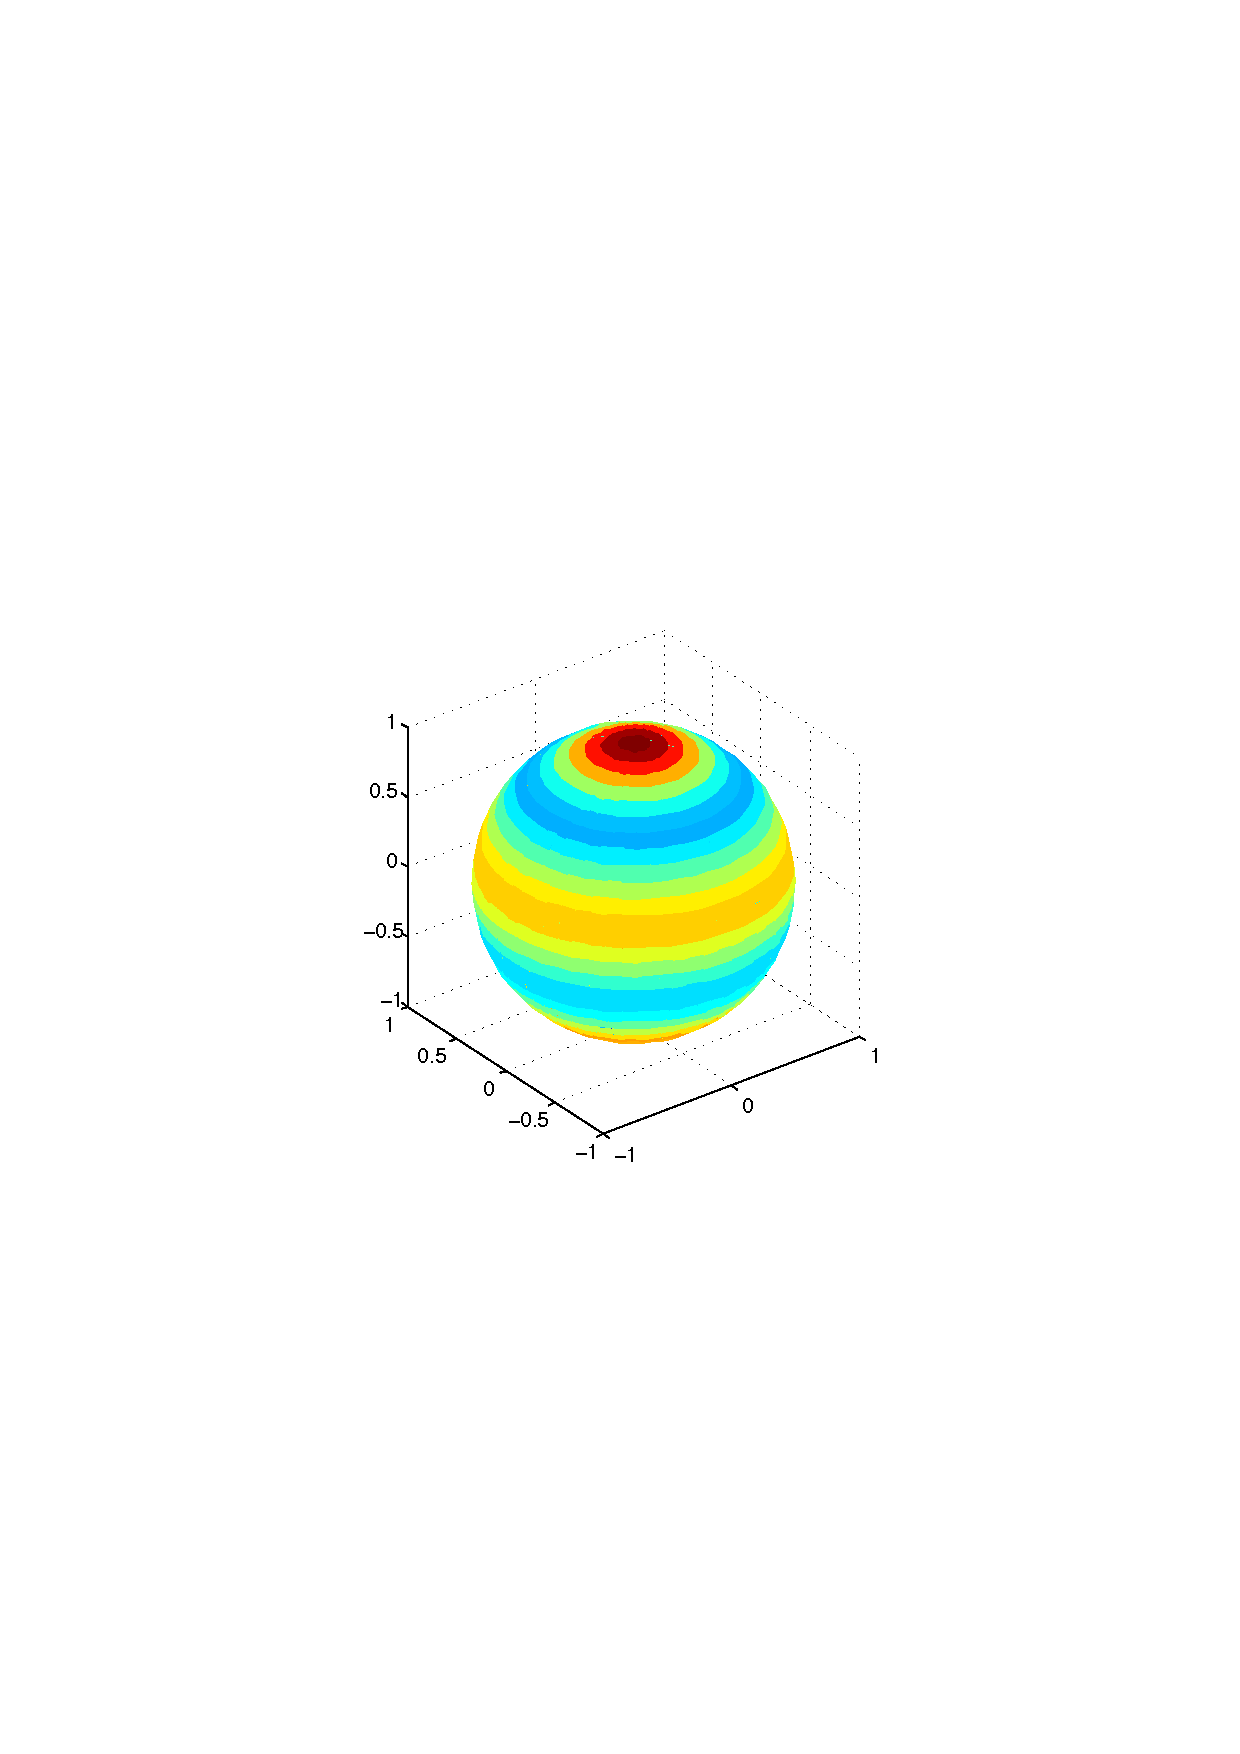
\includegraphics[width=0.45\textwidth]{kugel/ylm/a_5_0.pdf}
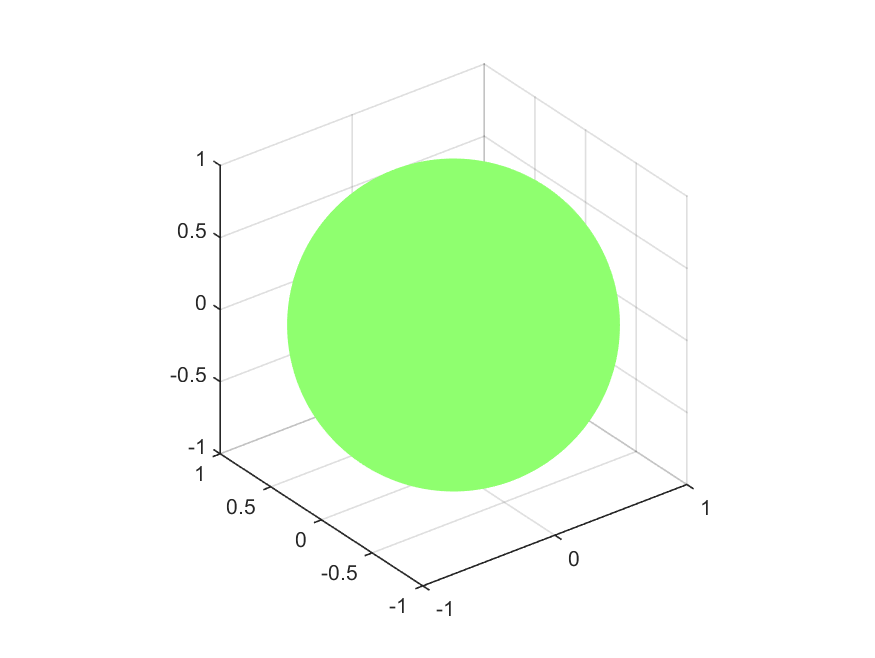
\includegraphics[width=0.45\textwidth]{kugel/ylm/b_5_0.pdf}
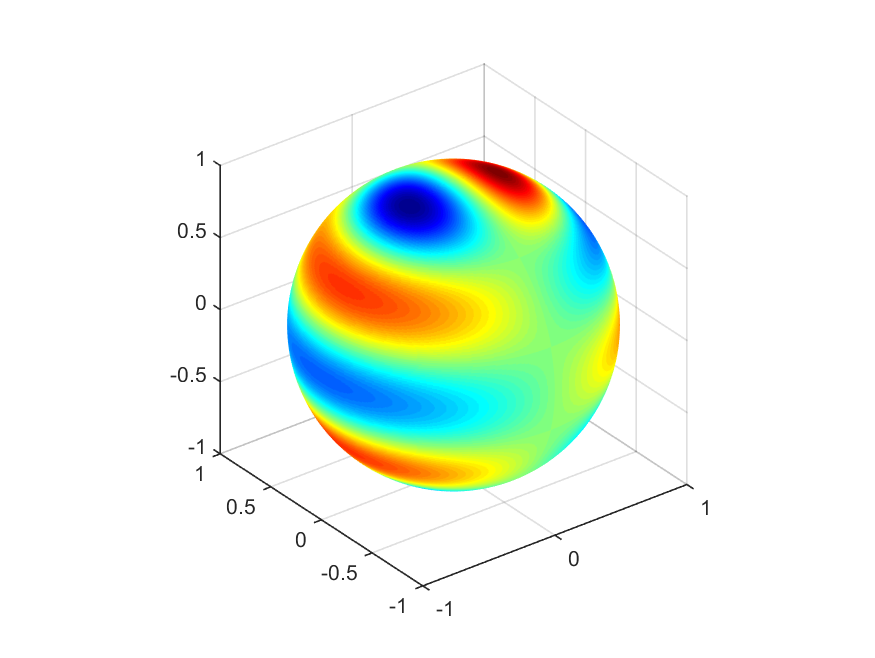
\includegraphics[width=0.45\textwidth]{kugel/ylm/a_5_1.pdf}
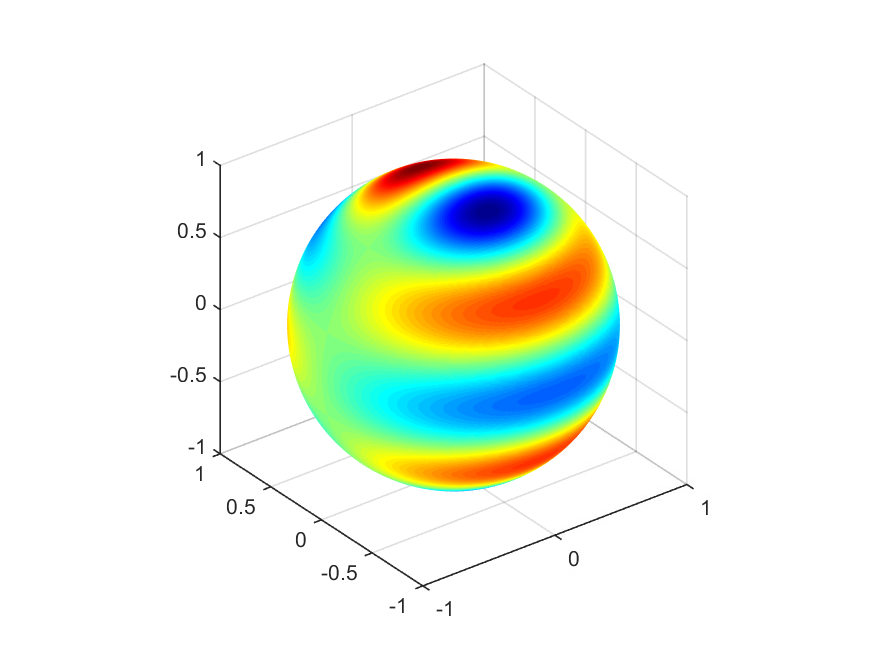
\includegraphics[width=0.45\textwidth]{kugel/ylm/b_5_1.pdf}
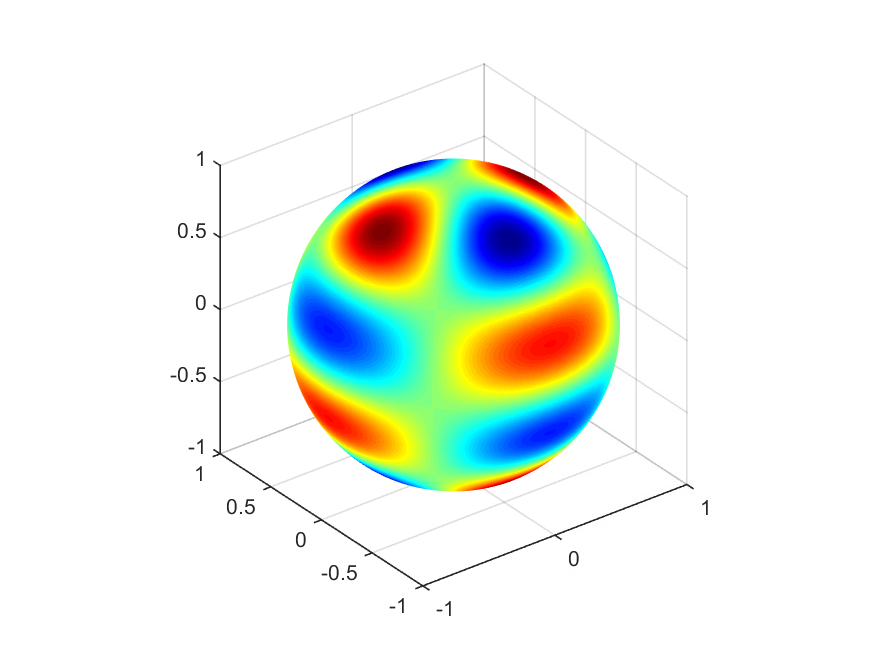
\includegraphics[width=0.45\textwidth]{kugel/ylm/a_5_2.pdf}
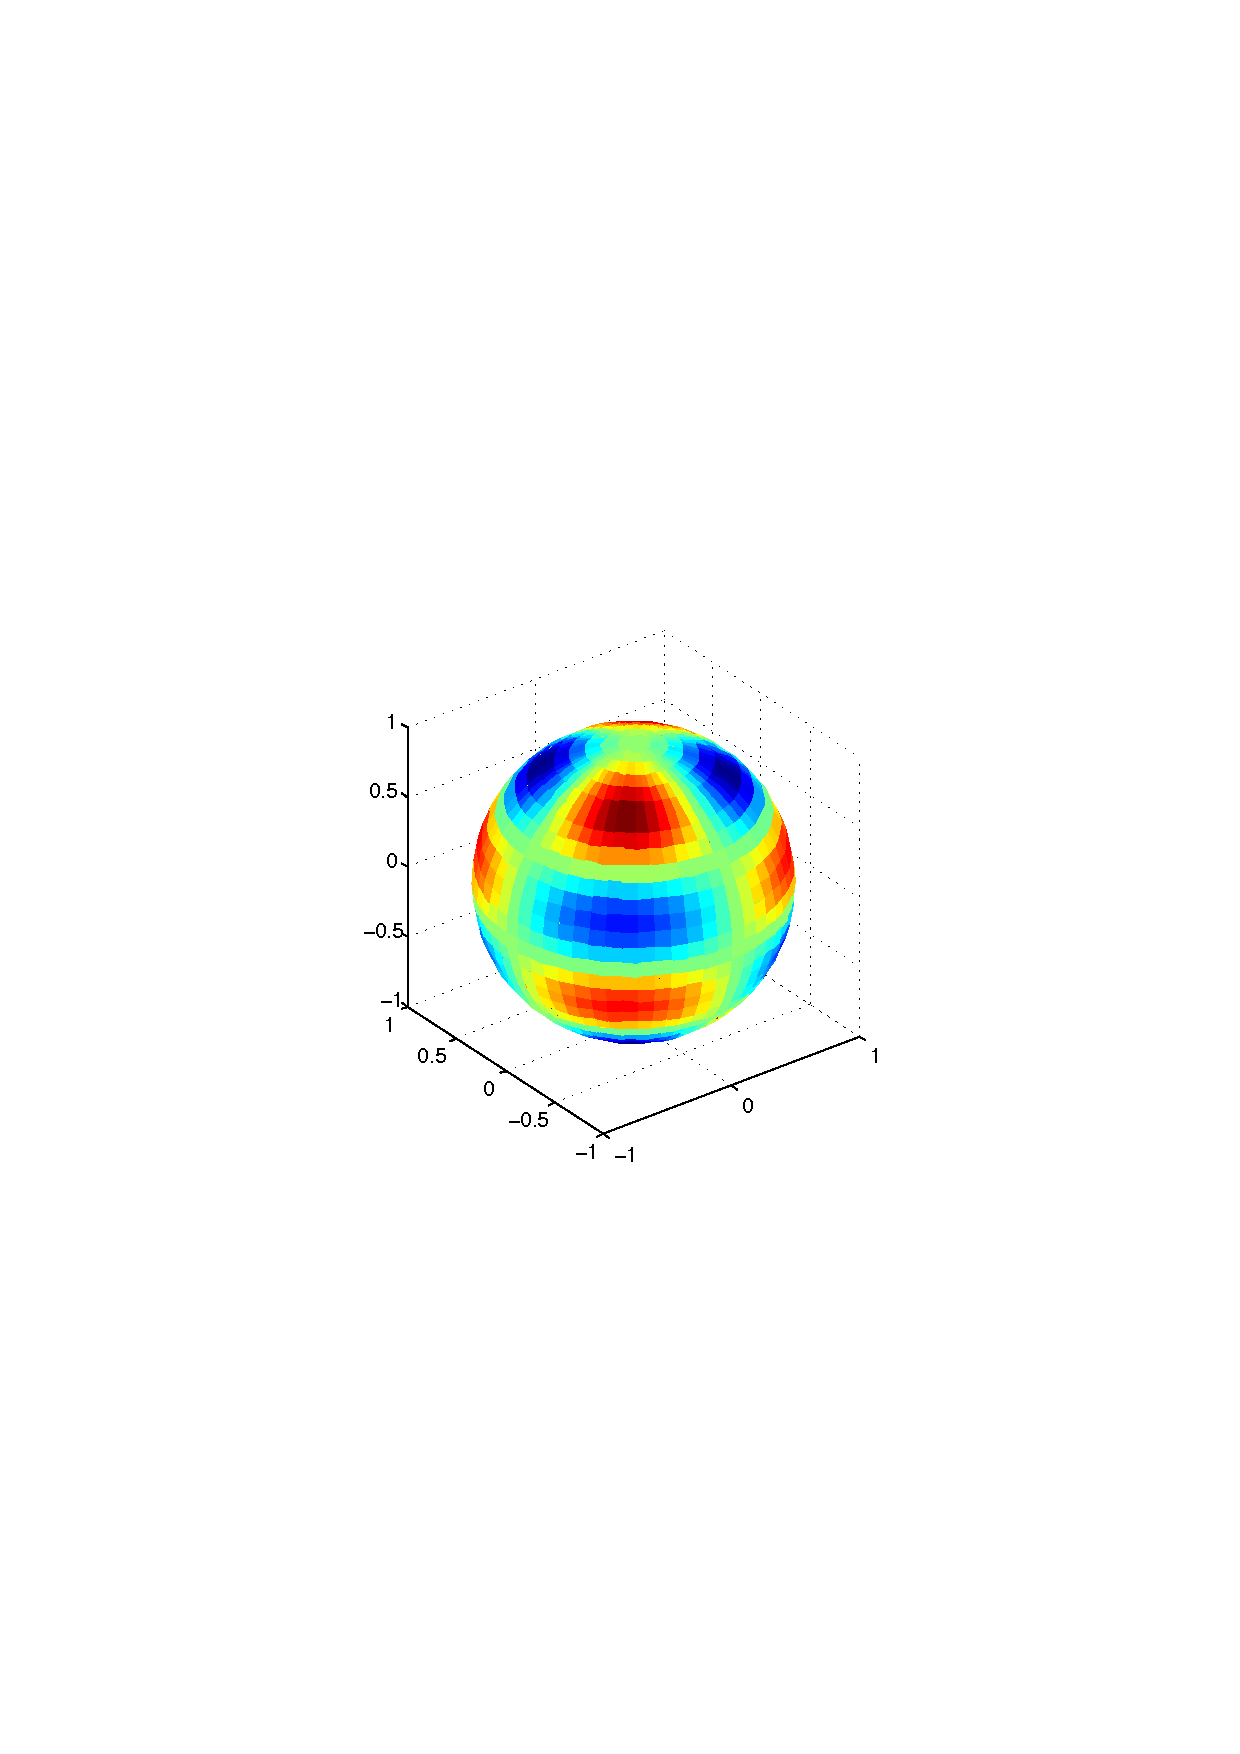
\includegraphics[width=0.45\textwidth]{kugel/ylm/b_5_2.pdf}
\caption{$Y_{lm}$ mit $l=5$, $m=0$, 1, 2 $\&$ $Z_{lm}$ mit $l=5$, $m=0$, 1, 2
\label{skript:Bild 0}}
\end{figure}

\begin{figure}% Bilder 3-5 Y_lm und Z_lm
\centering
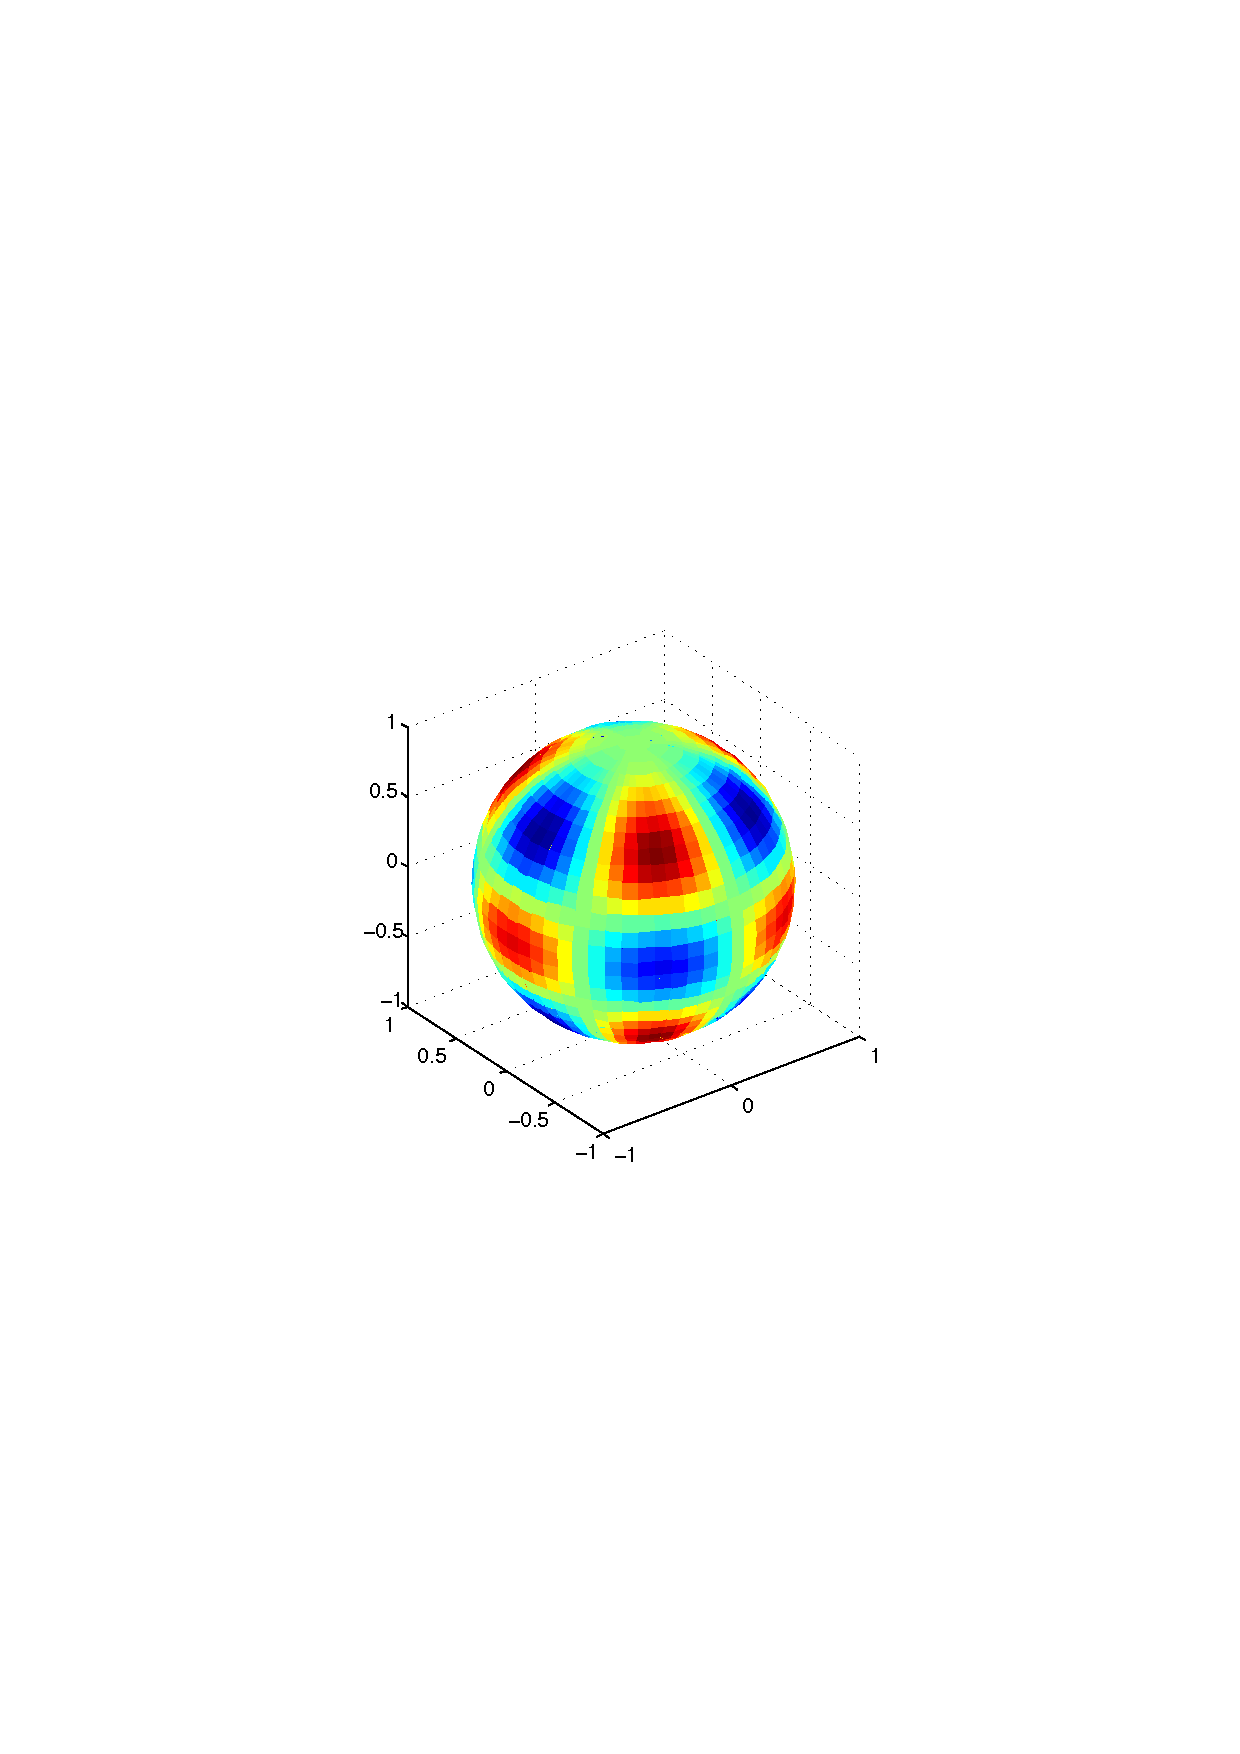
\includegraphics[width=0.45\textwidth]{kugel/ylm/a_5_3.pdf}
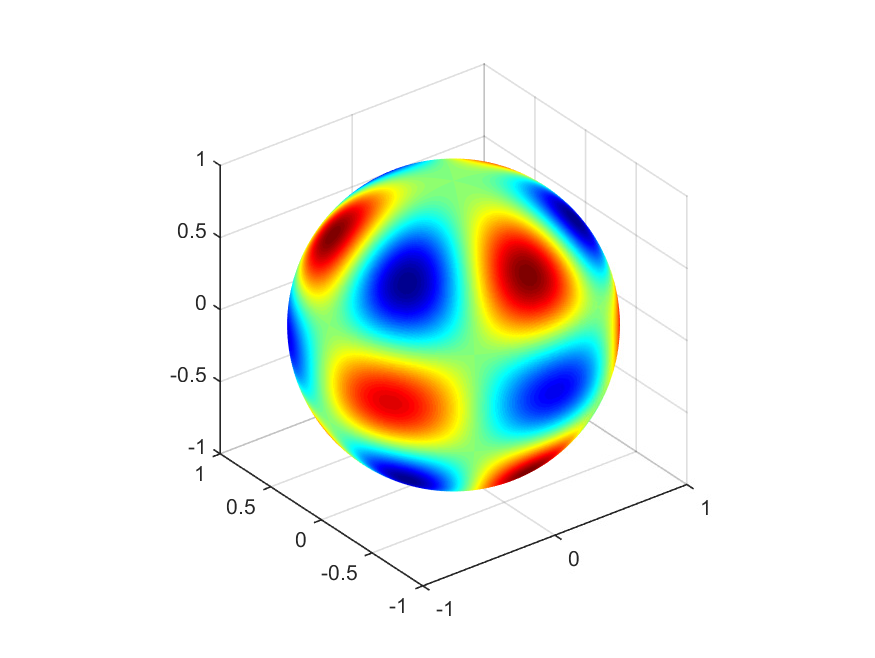
\includegraphics[width=0.45\textwidth]{kugel/ylm/b_5_3.pdf}
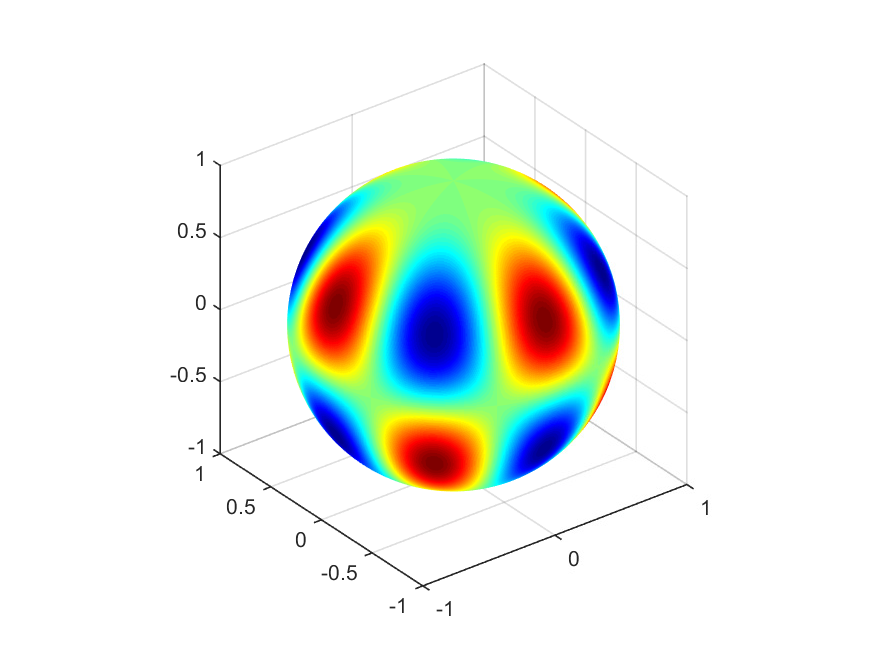
\includegraphics[width=0.45\textwidth]{kugel/ylm/a_5_4.pdf}
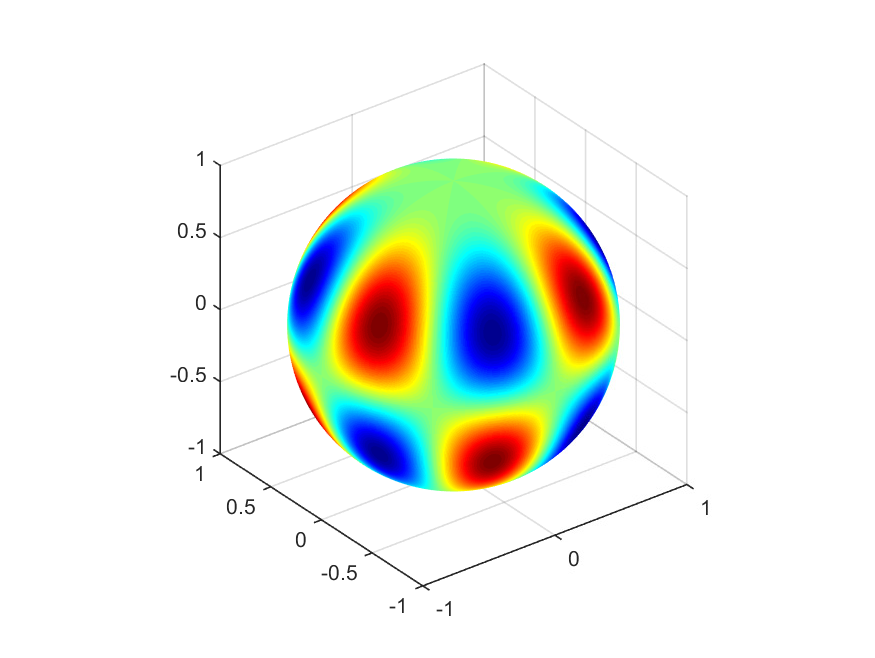
\includegraphics[width=0.45\textwidth]{kugel/ylm/b_5_4.pdf}
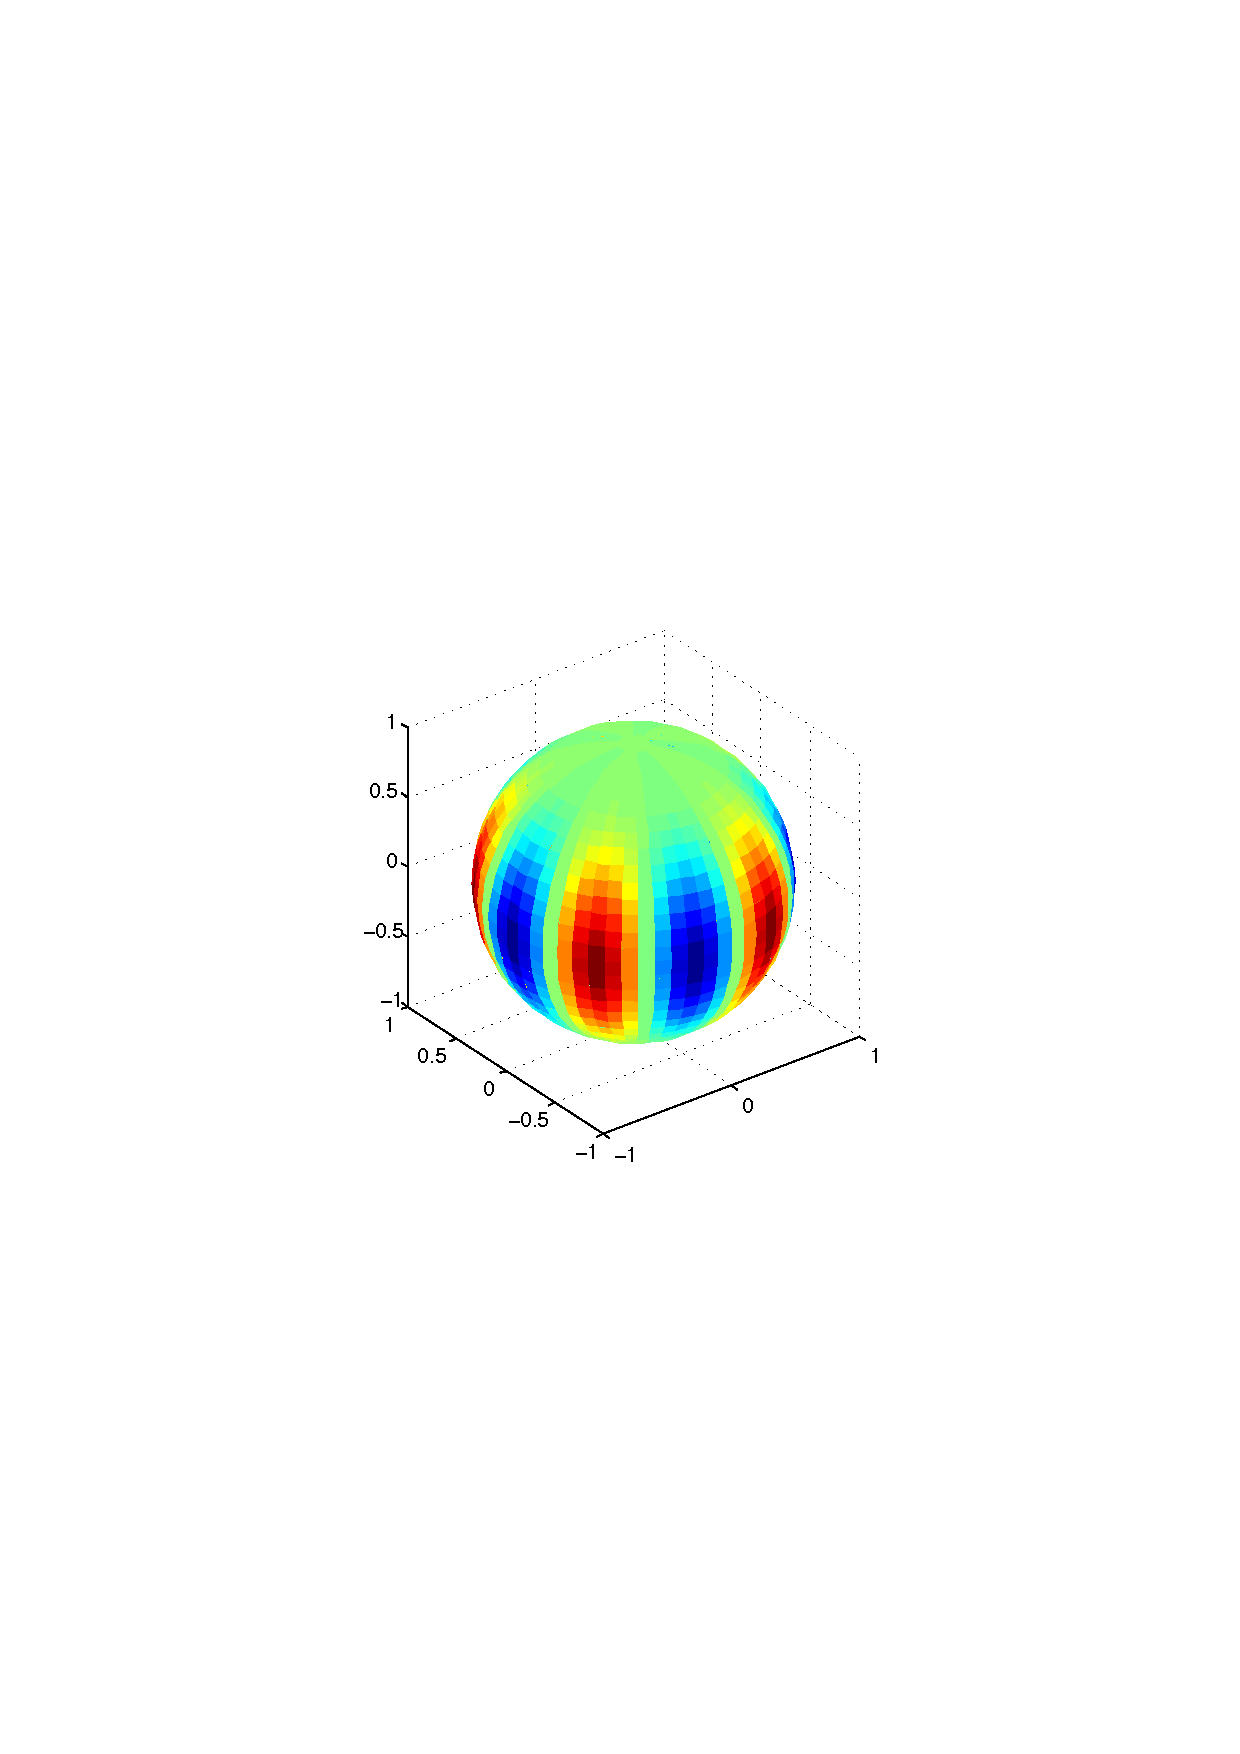
\includegraphics[width=0.45\textwidth]{kugel/ylm/a_5_5.pdf}
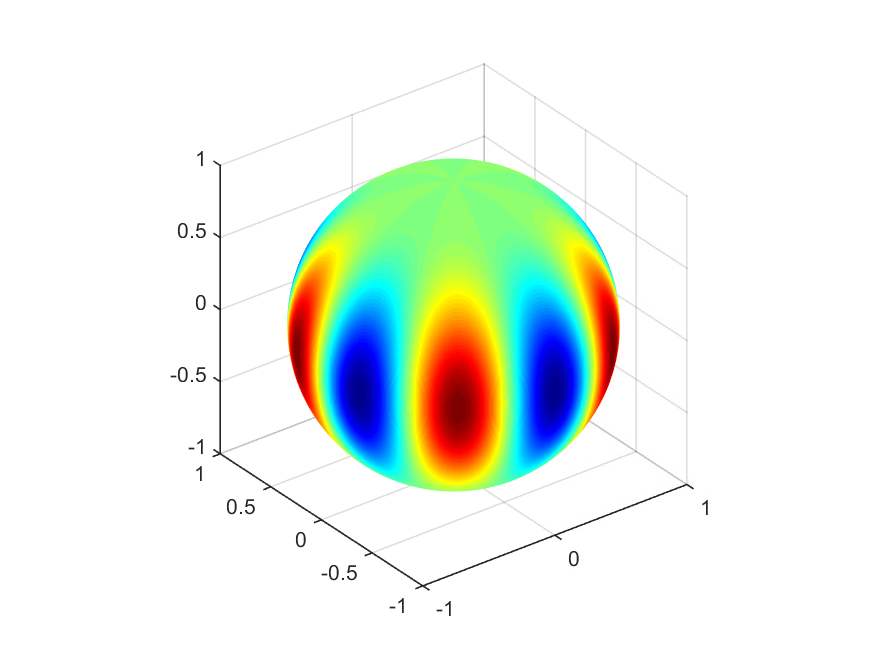
\includegraphics[width=0.45\textwidth]{kugel/ylm/b_5_5.pdf}
\caption{$Y_{lm}$ mit $l=5$, $m=3$, 4, 5 $\&$ $Z_{lm}$ mit $l=5$, $m=3$, 4, 5
\label{skript:Bild 2}}
\end{figure}

\section{Berechnung der Fourier-Koeffizienten auf der Kugeloberfl"ache} 
\rhead{Berechnung der Fourier-Koeffizienten auf der Kugeloberfläche}
\begin{align*}
\text{l=0} \qquad a_{00}&=\frac{1}{4\pi} \int_{-\pi}^\pi \int_{0}^\pi f(\vartheta,\varphi) \cdot \sin\vartheta \cdot d\vartheta \cdot d\varphi
\\
\text{l$\neq$0} \qquad a_{lm}&=\frac{1}{4\pi} \int_{-\pi}^\pi \int_{0}^\pi f(\vartheta,\varphi) \cdot Y_{lm} (\vartheta, \varphi) \cdot \sin\varphi \cdot d\vartheta \cdot d\varphi
\\
b_{lm}&=\frac{1}{4\pi} \int_{-\pi}^\pi \int_{0}^\pi f(\vartheta,\varphi) \cdot Z_{lm} (\vartheta, \varphi) \cdot \sin\varphi \cdot d\vartheta \cdot d\varphi
\end{align*}

\section{Zusammenfassen der Koeffizienten} 
\rhead{Zusammenfassen der Koeffizienten}
F"ur die Darstellung des komplexen Amplitudenspektrums muss man in der klassischen Fourier-Theorie die Sinus- und Kosinus-Koeffizienten noch zusammenfassen. Bei der Fourier-Theorie auf der Kugeloberfl"ache muss man die Koeffizienten folgendermassen zusammenfassen:
\begin{align*}
c_l=\sum_{m=0}^l \sqrt{a^2_{lm}+b^2_{lm}}
\end{align*}

\section{Konstantes komplexes Amplitudenspektrum}
\rhead{Konstantes komplexes Amplitudenspektrum}

In der nachfolgenden Bilderreihe kann man sehen dass, egal wo ein Signal auftritt, das komplexe Amplitudenspektrum in jedem Fall gleich bleibt.\\

(Bilder Rechteckfunktion und Kugel)
\begin{figure}
\centering
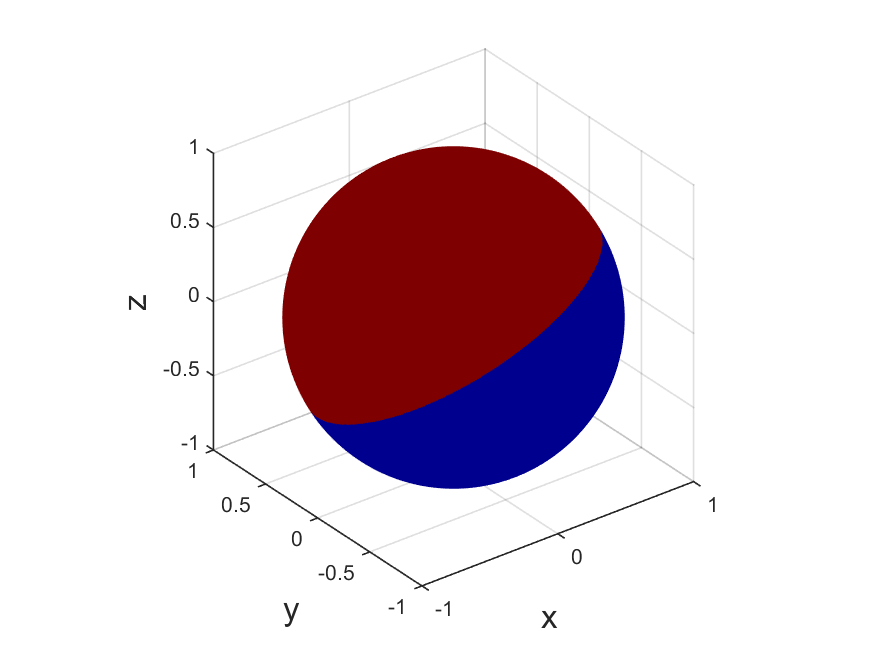
\includegraphics[width=0.49\textwidth]{kugel/kSpektrum/Kugel_1_1.pdf}
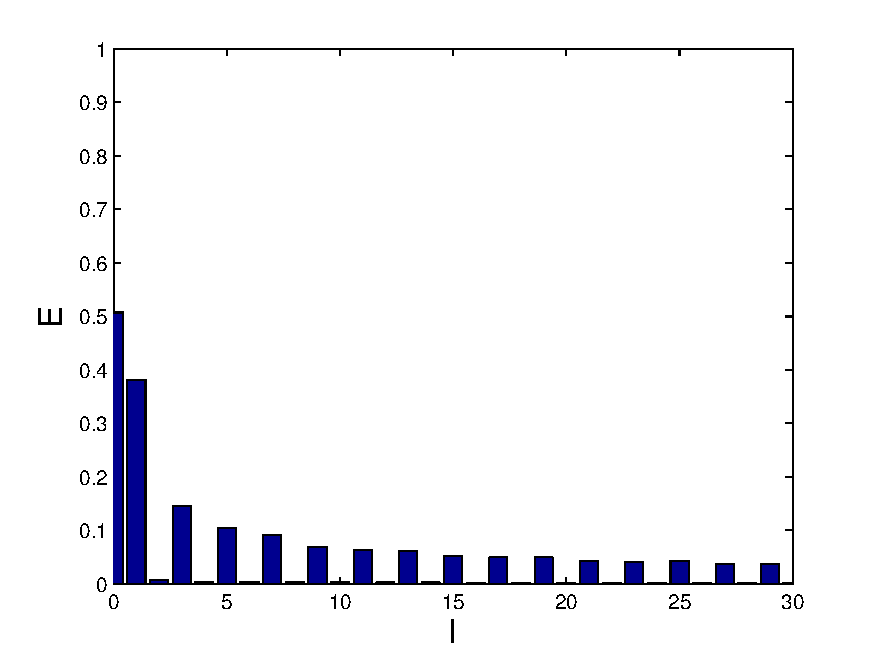
\includegraphics[width=0.49\textwidth]{kugel/kSpektrum/Kugel_1_2.pdf}
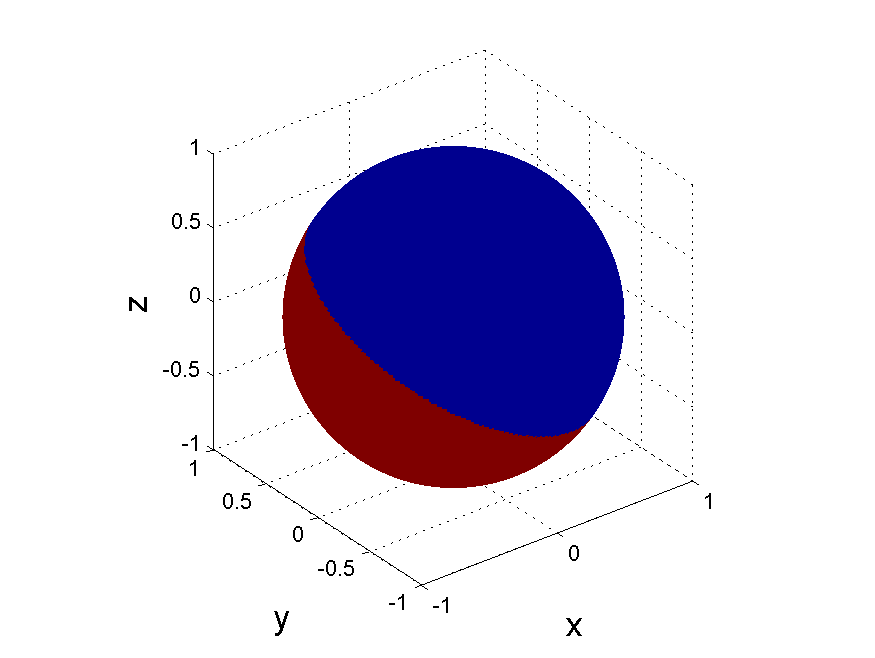
\includegraphics[width=0.49\textwidth]{kugel/kSpektrum/Kugel_2_1.pdf}
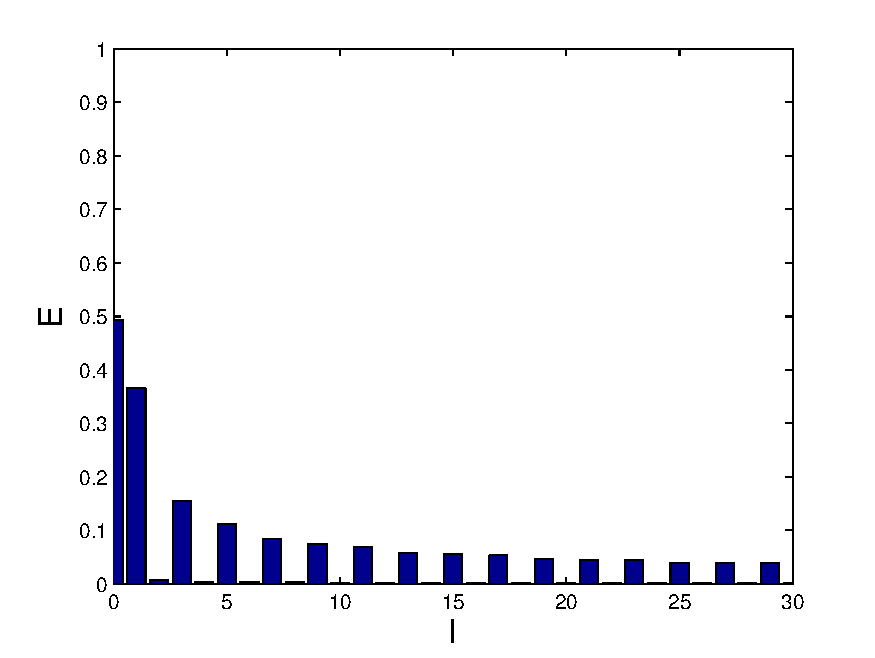
\includegraphics[width=0.49\textwidth]{kugel/kSpektrum/Kugel_2_2.pdf}
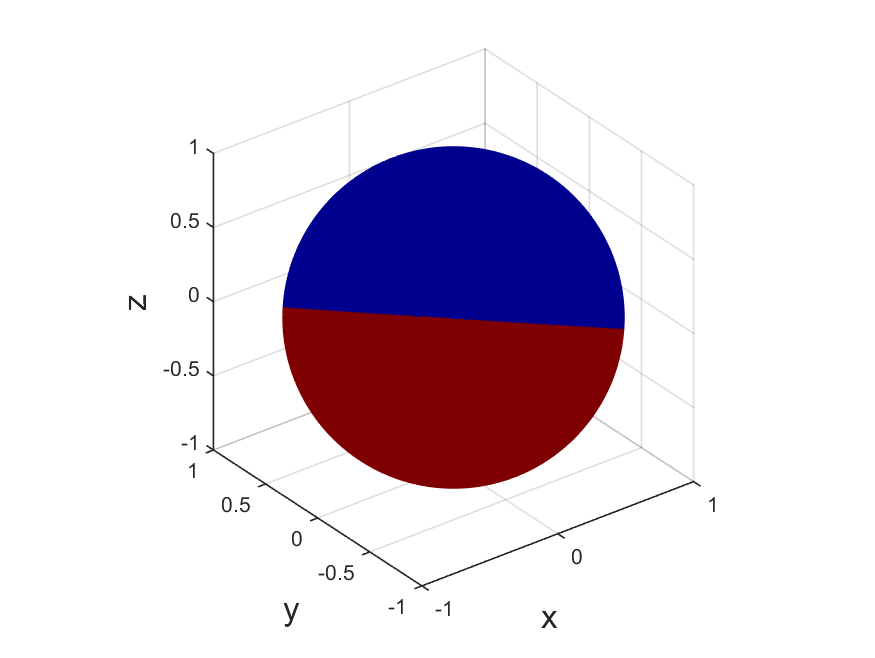
\includegraphics[width=0.49\textwidth]{kugel/kSpektrum/Kugel_3_1.pdf}
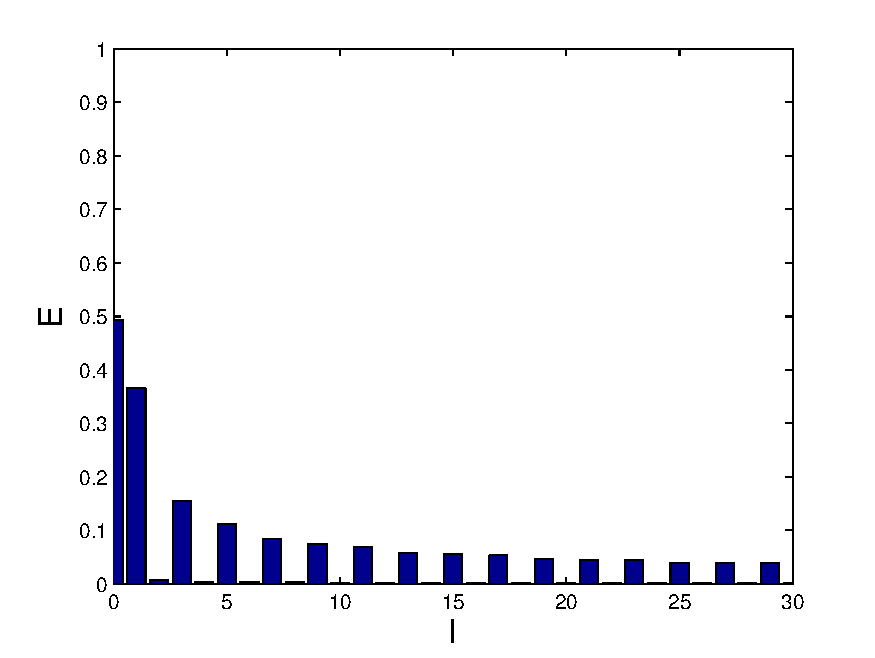
\includegraphics[width=0.49\textwidth]{kugel/kSpektrum/Kugel_3_2.pdf}
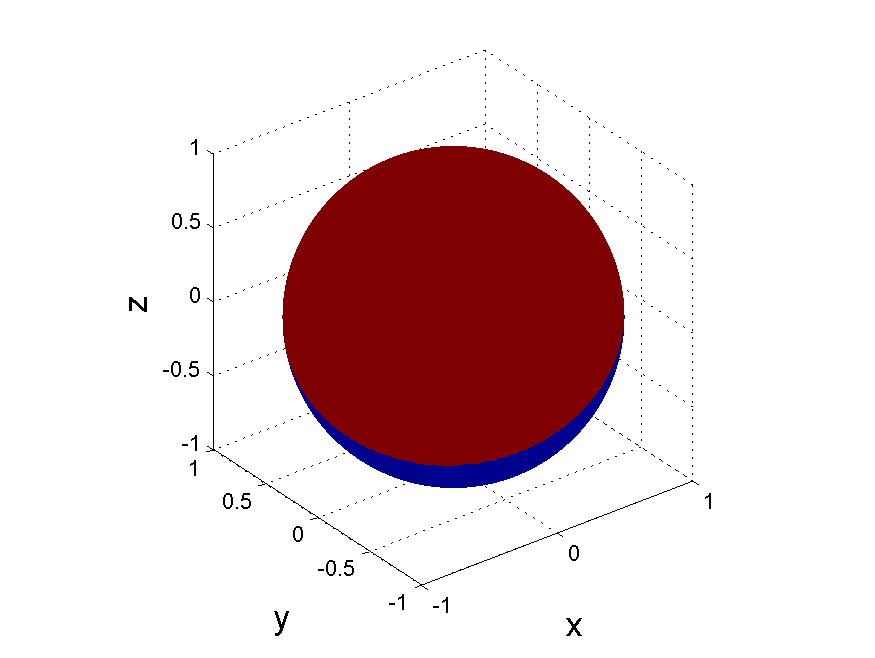
\includegraphics[width=0.49\textwidth]{kugel/kSpektrum/Kugel_4_1.pdf}
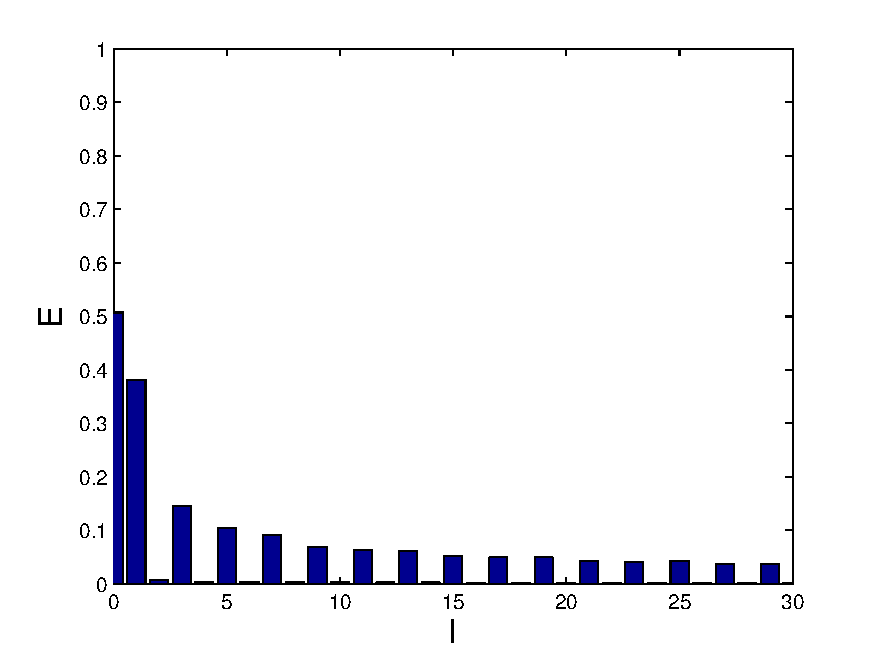
\includegraphics[width=0.49\textwidth]{kugel/kSpektrum/Kugel_4_2.pdf}
\caption{Titel??
\label{skript:Spektrum1}}
\end{figure}

\begin{figure}
\centering
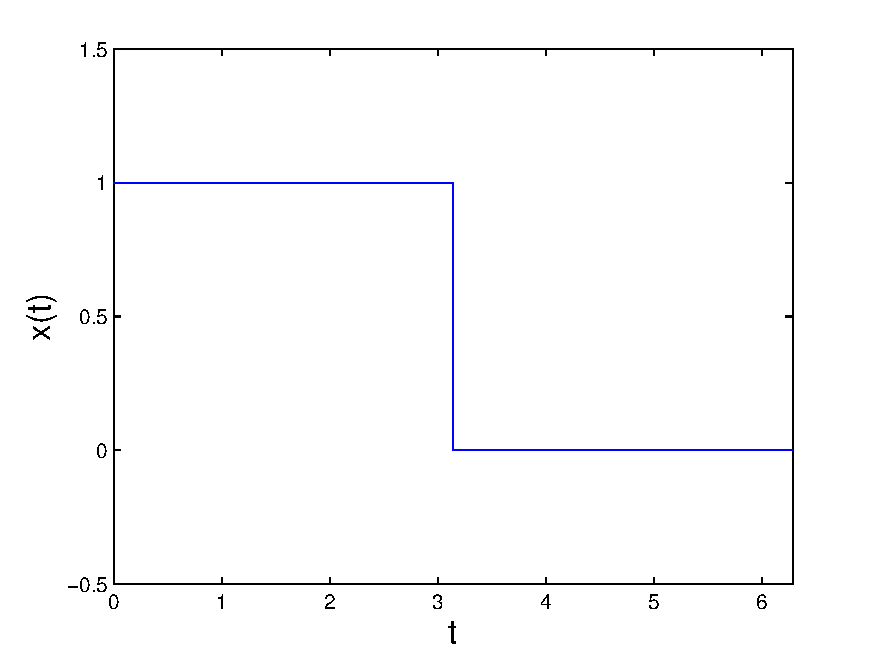
\includegraphics[width=0.49\textwidth]{kugel/kSpektrum/Rechteck1_1.pdf}
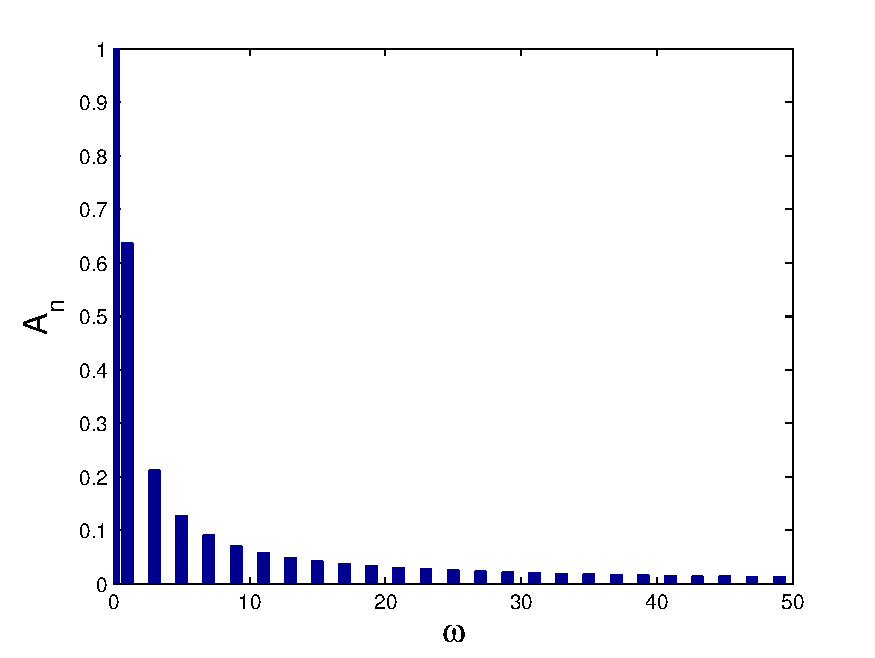
\includegraphics[width=0.49\textwidth]{kugel/kSpektrum/Rechteck1_2.pdf}
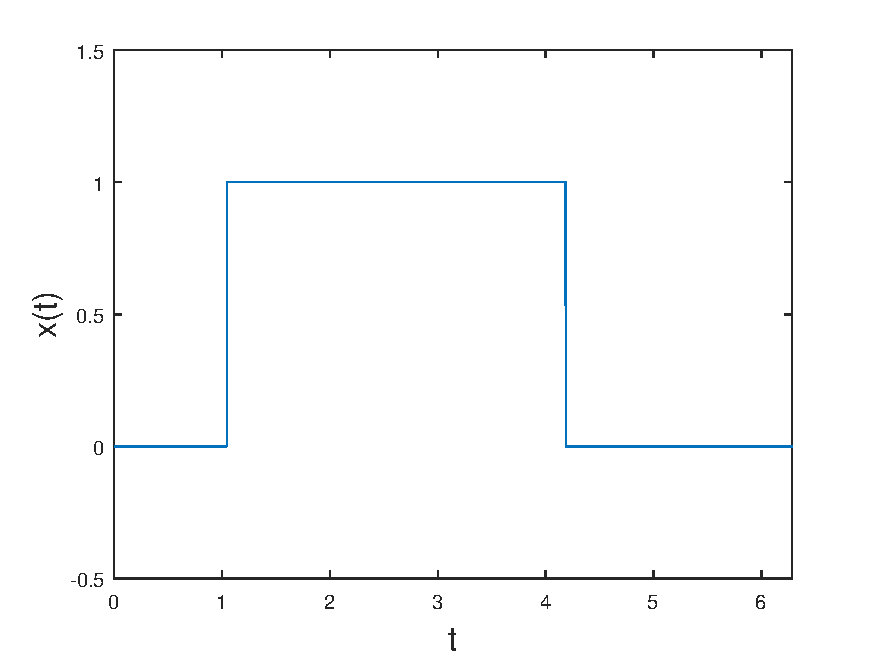
\includegraphics[width=0.49\textwidth]{kugel/kSpektrum/Rechteck2_1.pdf}
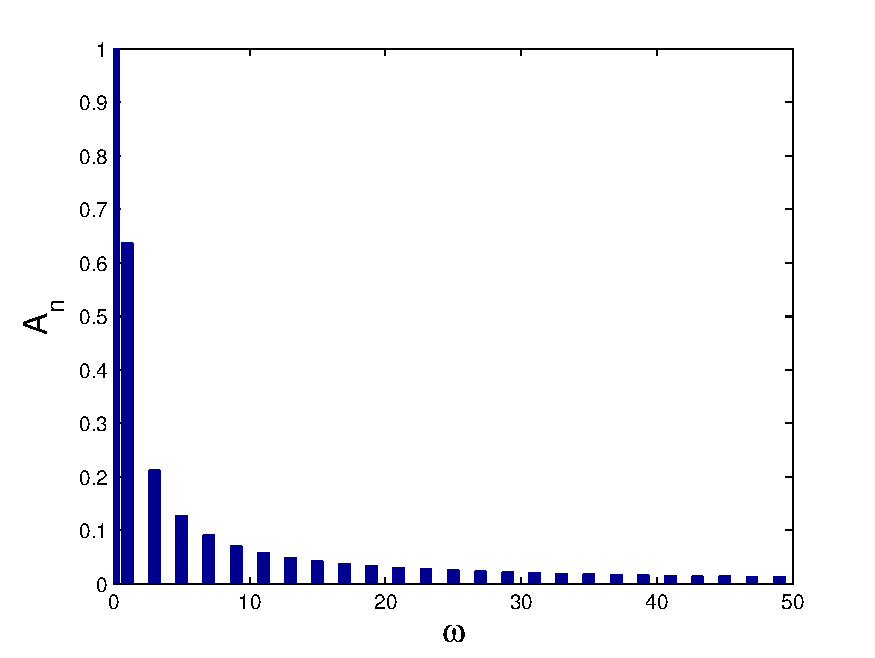
\includegraphics[width=0.49\textwidth]{kugel/kSpektrum/Rechteck1_2.pdf}
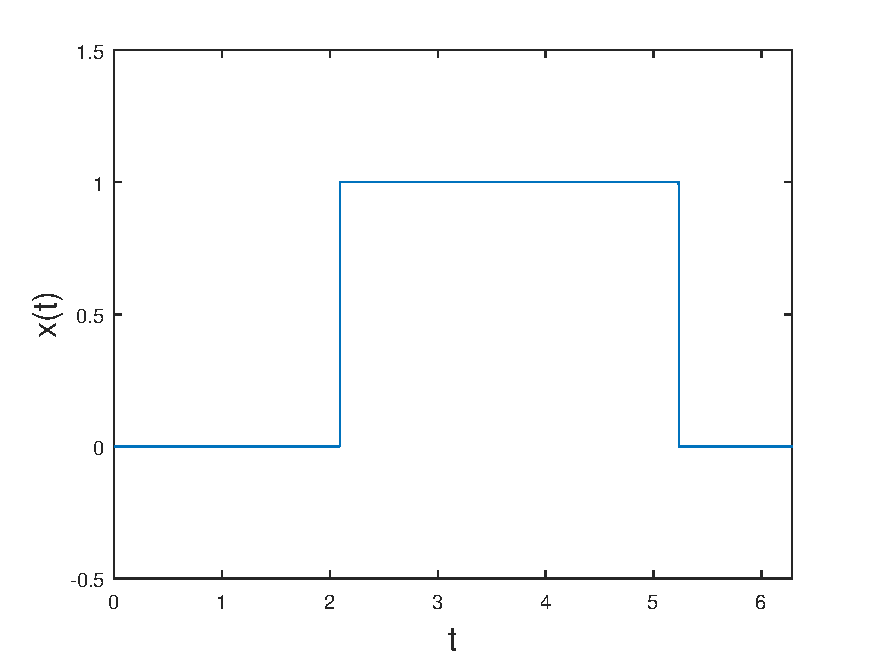
\includegraphics[width=0.49\textwidth]{kugel/kSpektrum/Rechteck3_1.pdf}
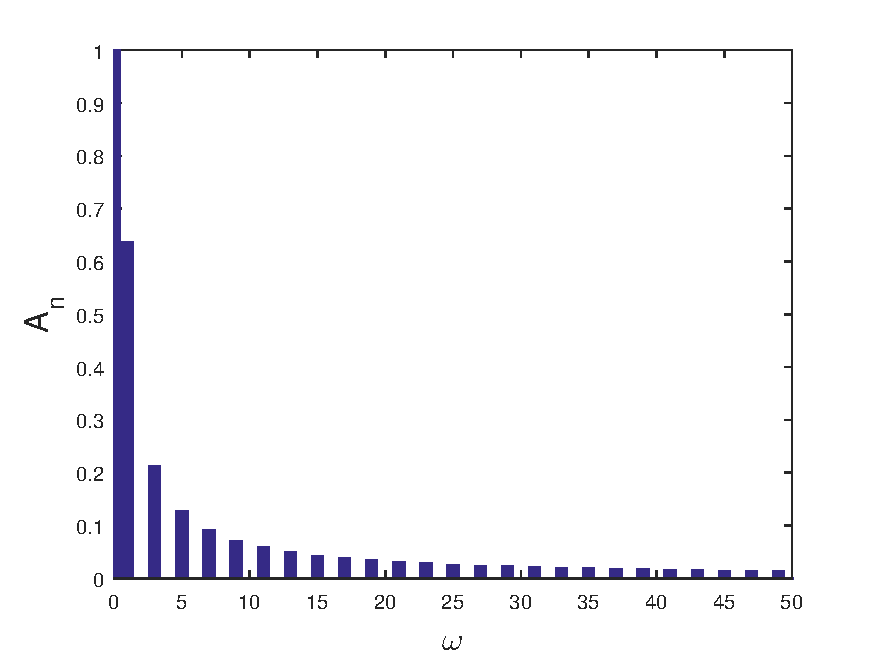
\includegraphics[width=0.49\textwidth]{kugel/kSpektrum/Rechteck3_2.pdf}
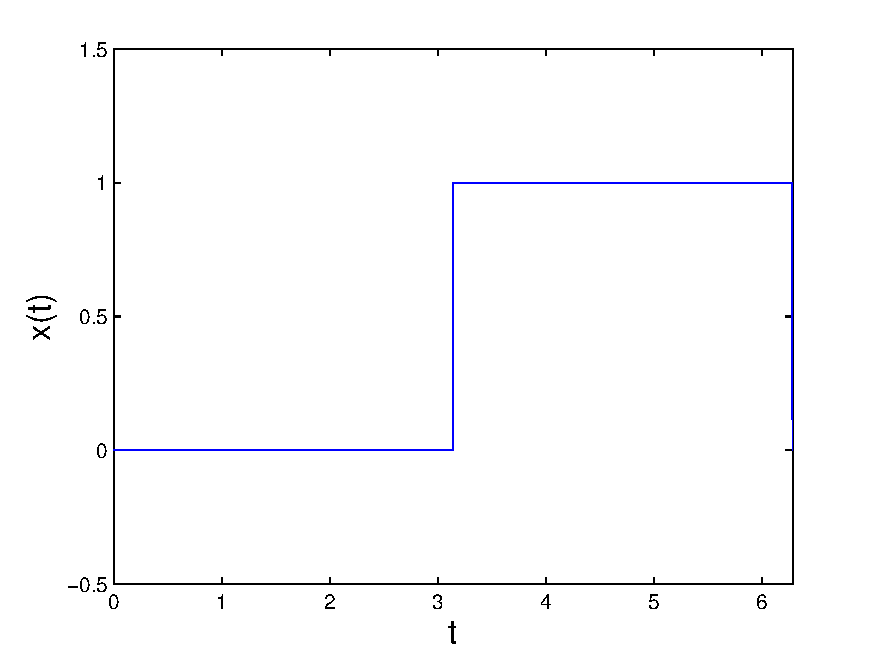
\includegraphics[width=0.49\textwidth]{kugel/kSpektrum/Rechteck4_1.pdf}
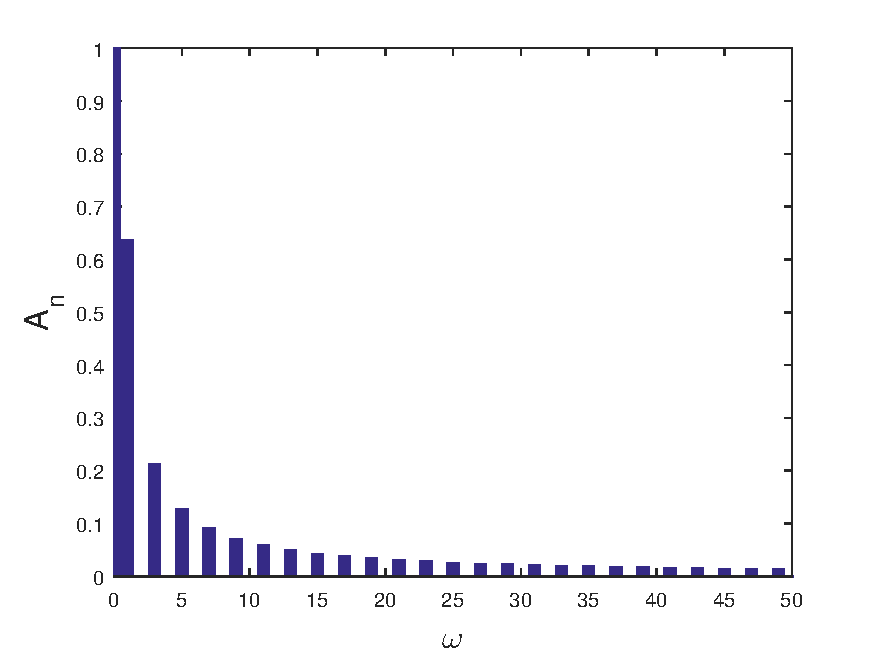
\includegraphics[width=0.49\textwidth]{kugel/kSpektrum/Rechteck4_2.pdf}
\caption{Titel??
\label{skript:Spektrum1}}
\end{figure}
\section{Vom Dirac-Stoss zu einer konstanten Funktion}
\rhead{Vom Dirac-Stoss zu einer konstanten Funktion}

Die folgende Bilderreihe zeigt auf, dass im Fall von einem Dirac-Stoss alle Frequenzen gleich stark vertreten sind. Hingegen im Fall einer konstant Funktion nur noch der 0-te Koeffizient Gewichtet ist.

\begin{figure}
\centering
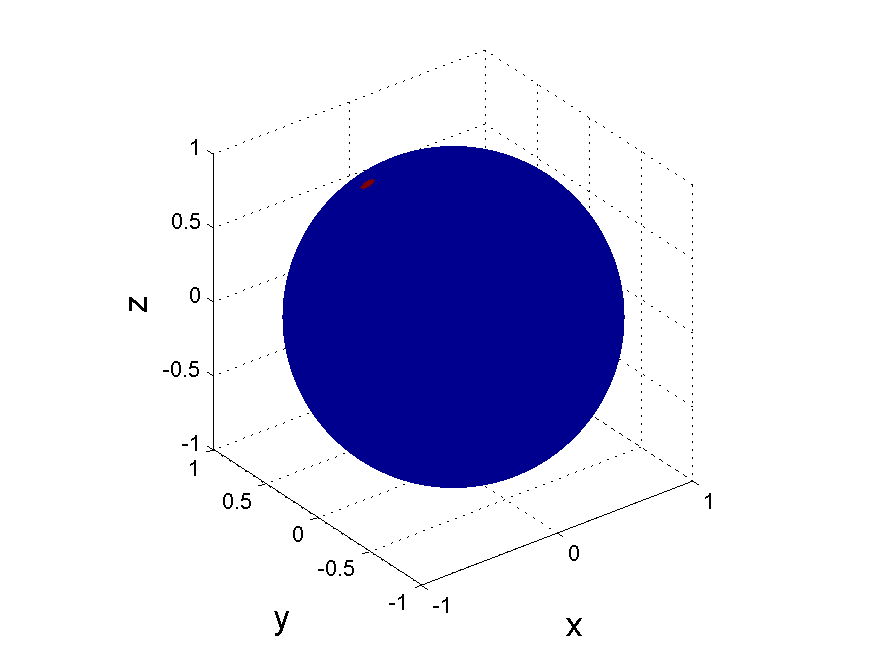
\includegraphics[width=0.49\textwidth]{kugel/Dkonstant/Kugel1_1.pdf}
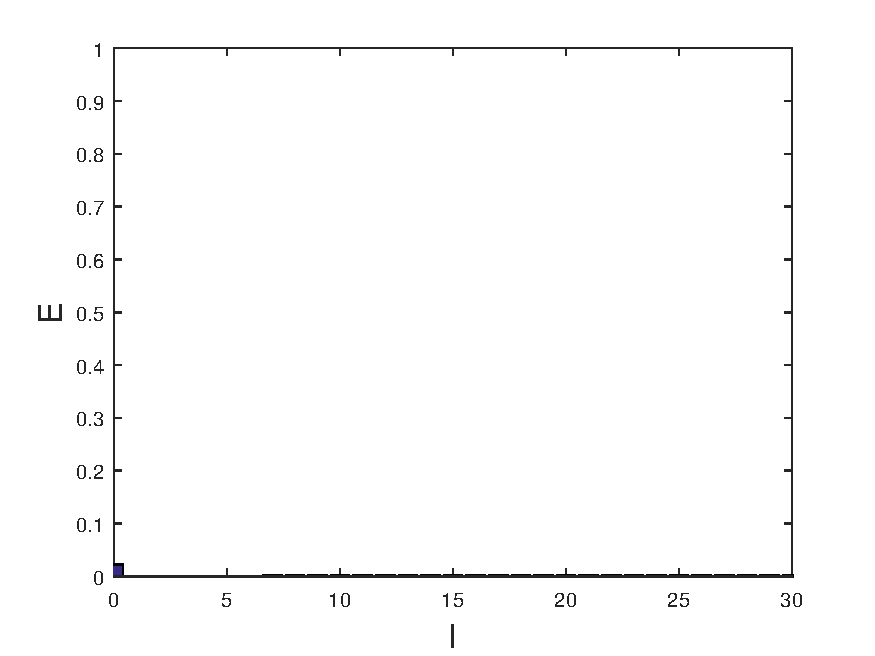
\includegraphics[width=0.49\textwidth]{kugel/Dkonstant/Kugel1_2.pdf}
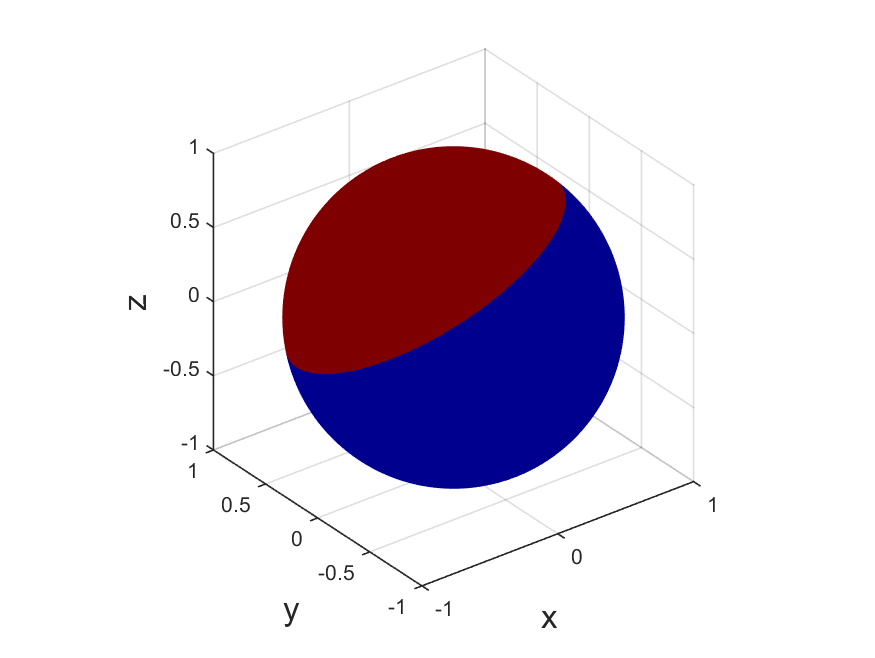
\includegraphics[width=0.49\textwidth]{kugel/Dkonstant/Kugel2_1.pdf}
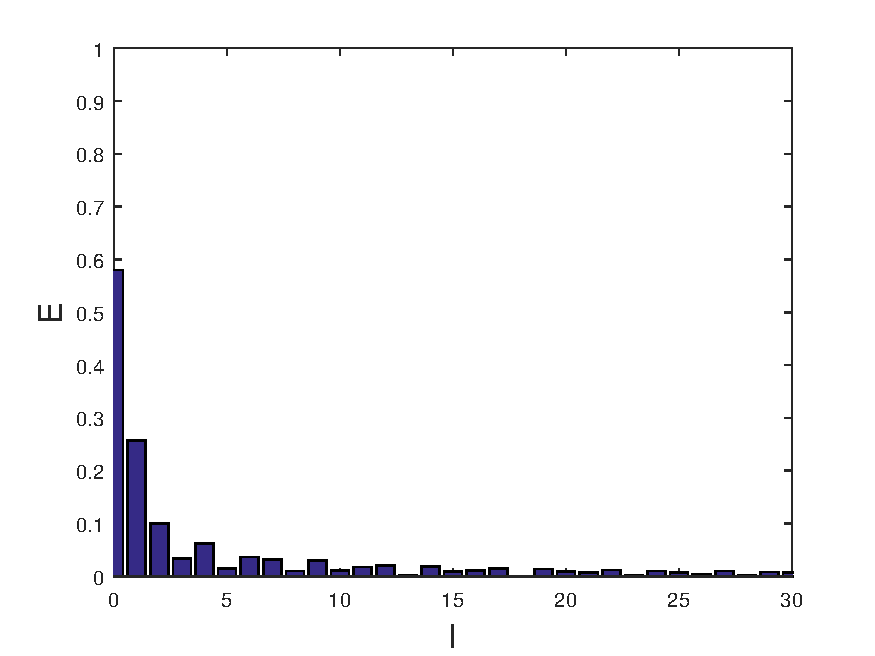
\includegraphics[width=0.49\textwidth]{kugel/Dkonstant/Kugel2_2.pdf}
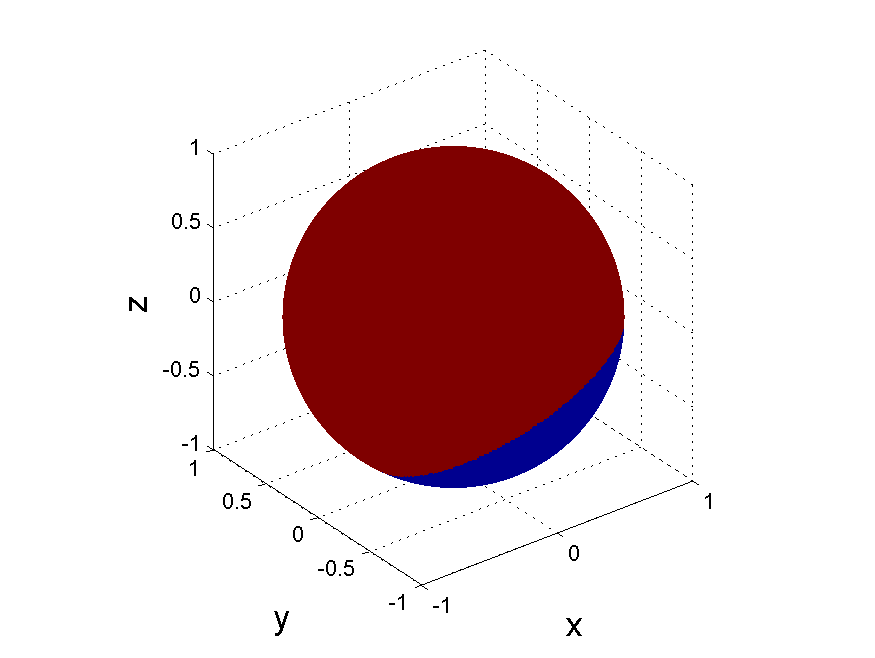
\includegraphics[width=0.49\textwidth]{kugel/Dkonstant/Kugel3_1.pdf}
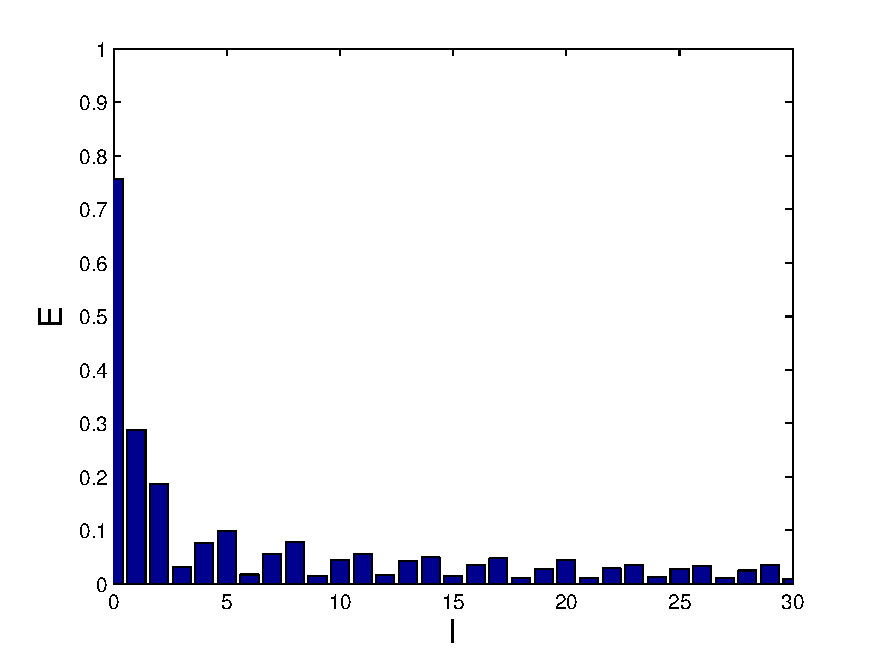
\includegraphics[width=0.49\textwidth]{kugel/Dkonstant/Kugel3_2.pdf}
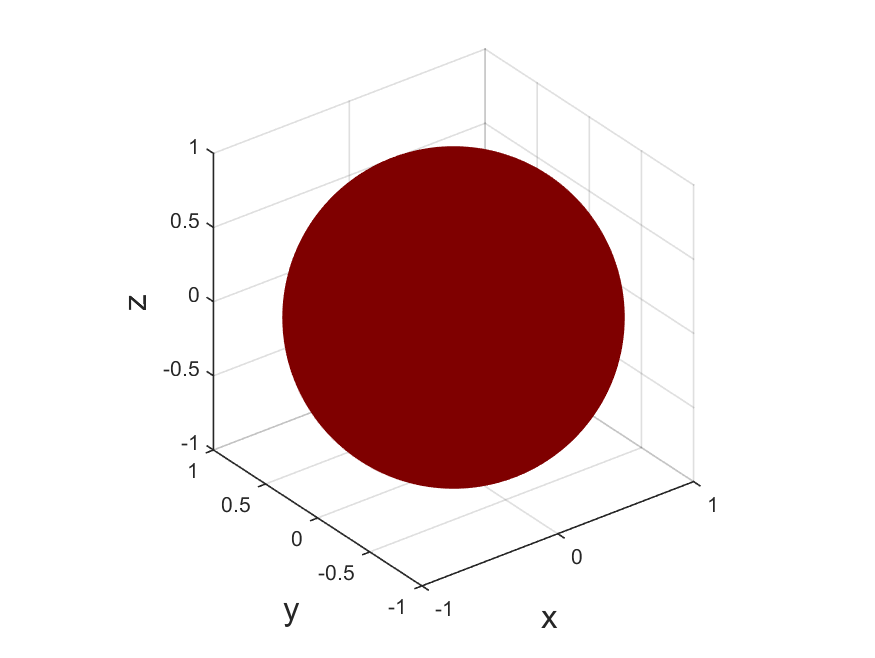
\includegraphics[width=0.49\textwidth]{kugel/Dkonstant/Kugel4_1.pdf}
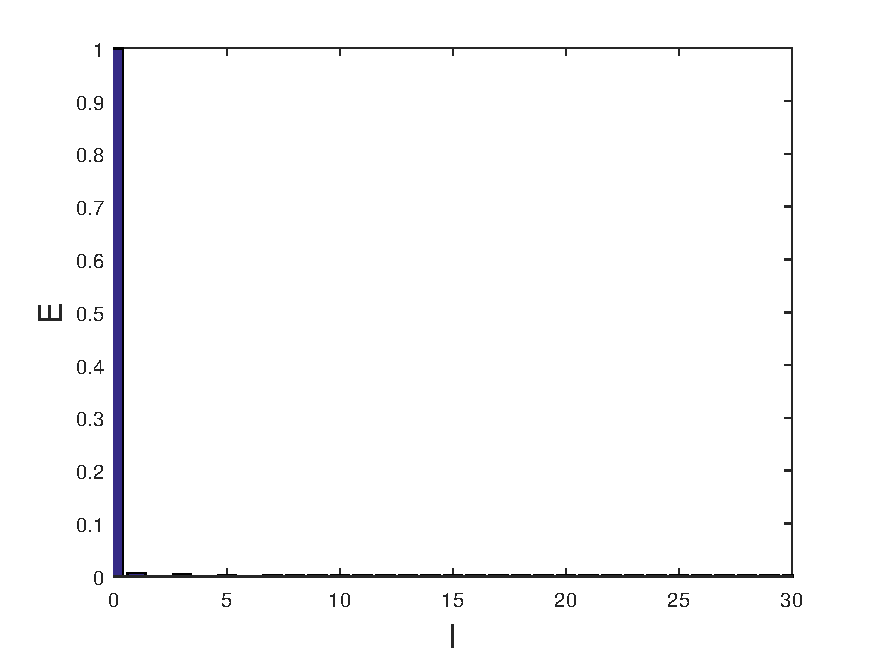
\includegraphics[width=0.49\textwidth]{kugel/Dkonstant/Kugel4_2.pdf}
\caption{Titel??
\label{skript:Dirac1}}
\end{figure}

\begin{figure}
\centering
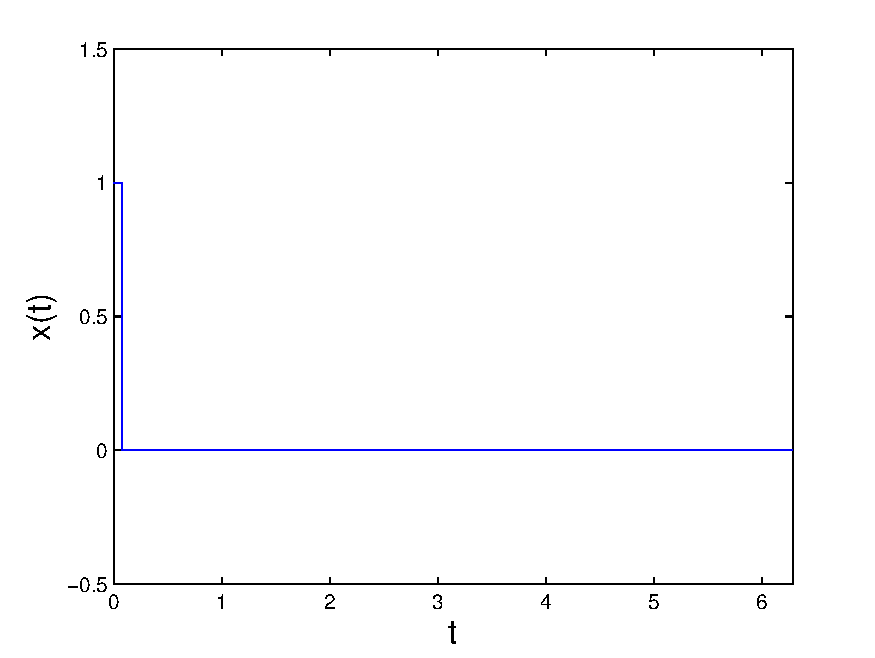
\includegraphics[width=0.49\textwidth]{kugel/Dkonstant/Rechteck1_1.pdf}
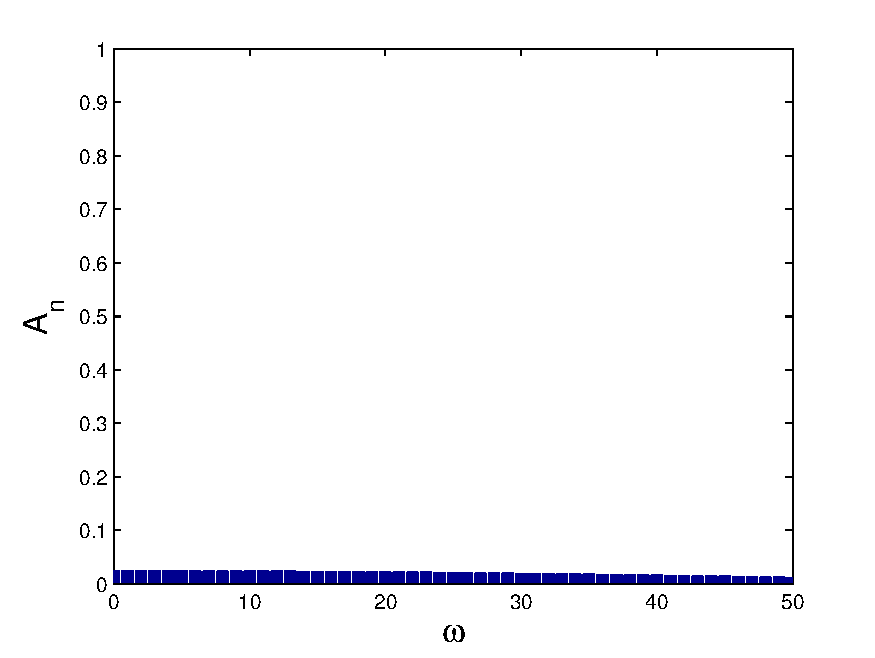
\includegraphics[width=0.49\textwidth]{kugel/Dkonstant/Rechteck1_2.pdf}
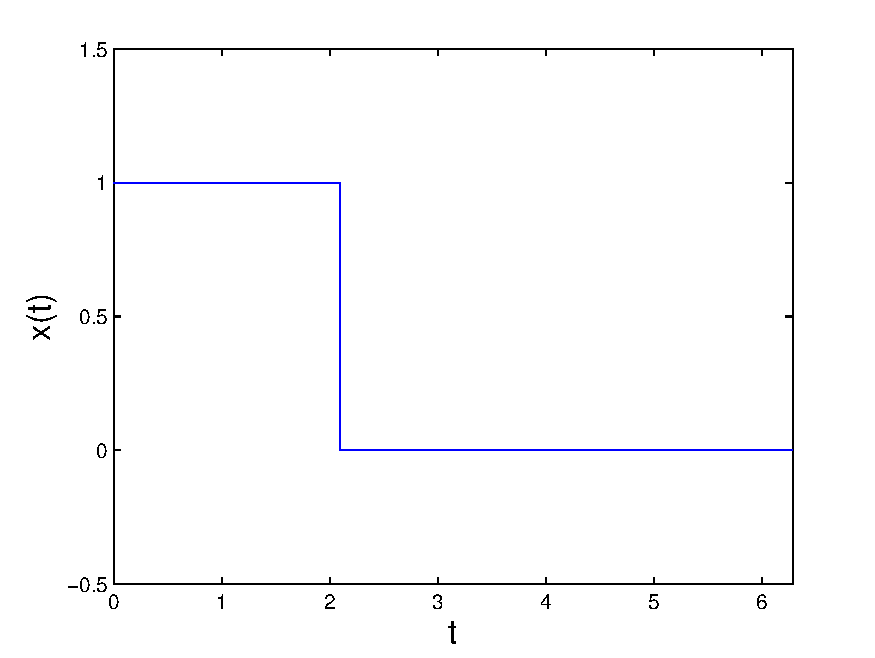
\includegraphics[width=0.49\textwidth]{kugel/Dkonstant/Rechteck2_1.pdf}
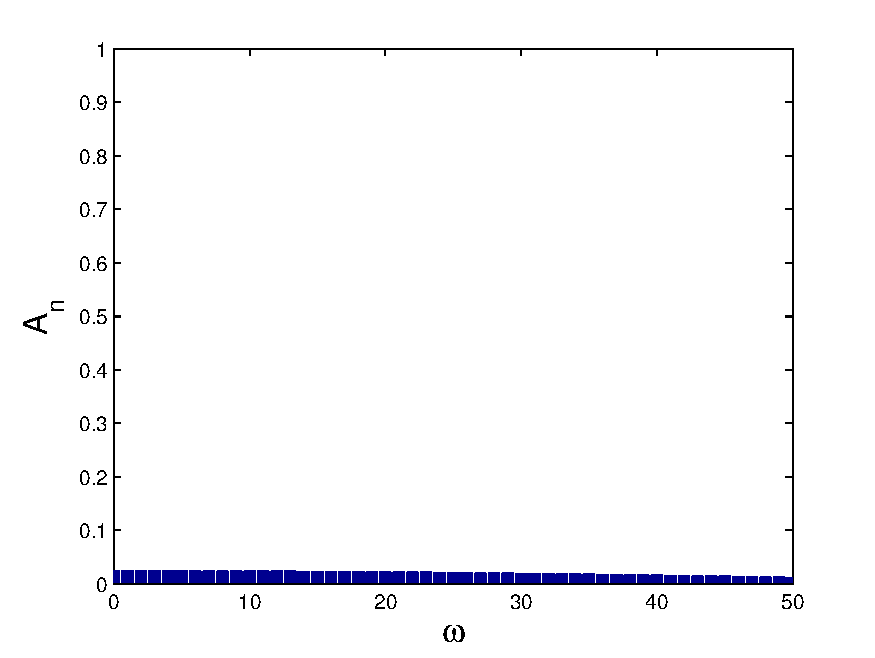
\includegraphics[width=0.49\textwidth]{kugel/Dkonstant/Rechteck1_2.pdf}
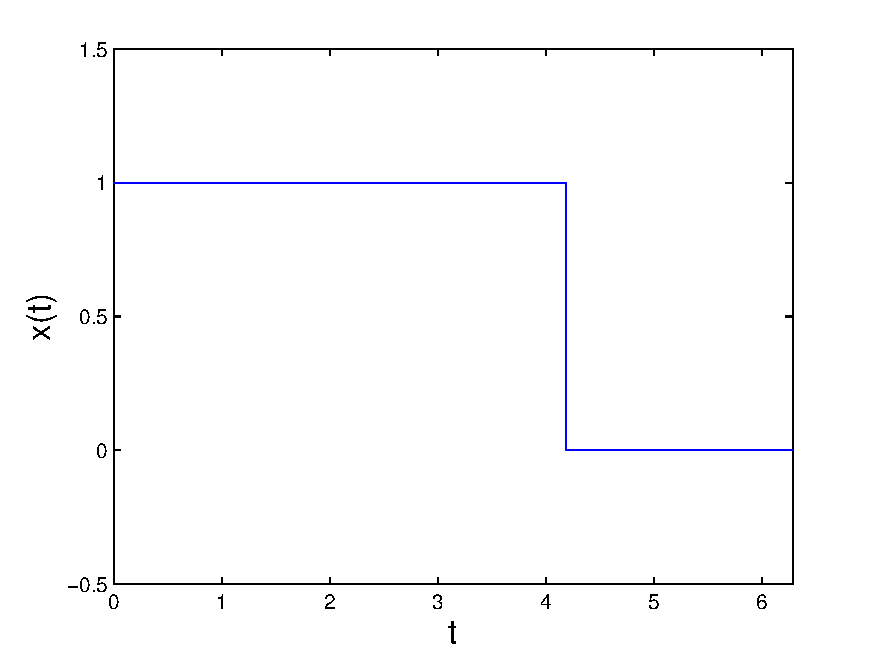
\includegraphics[width=0.49\textwidth]{kugel/Dkonstant/Rechteck3_1.pdf}
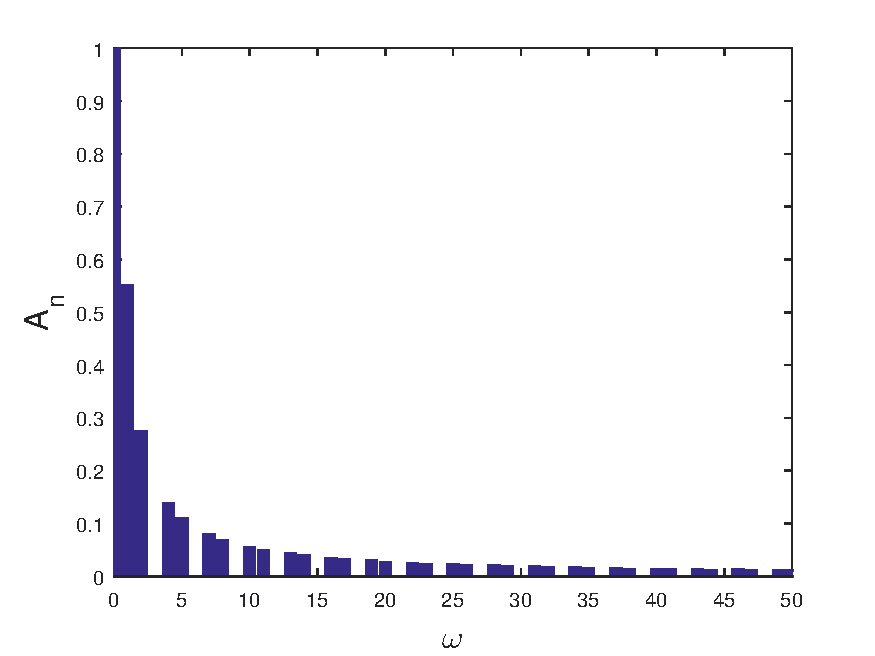
\includegraphics[width=0.49\textwidth]{kugel/Dkonstant/Rechteck3_2.pdf}
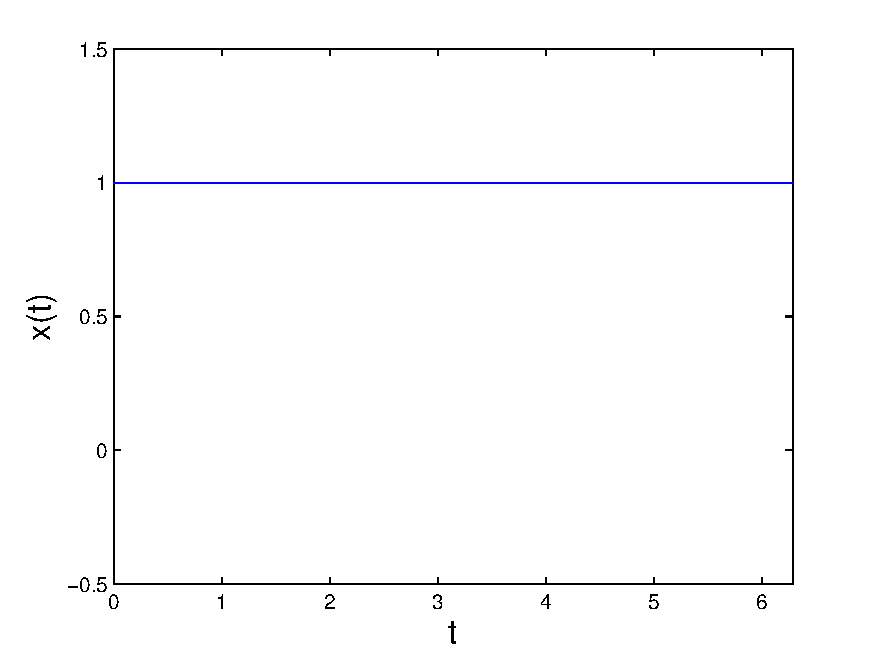
\includegraphics[width=0.49\textwidth]{kugel/Dkonstant/Rechteck4_1.pdf}
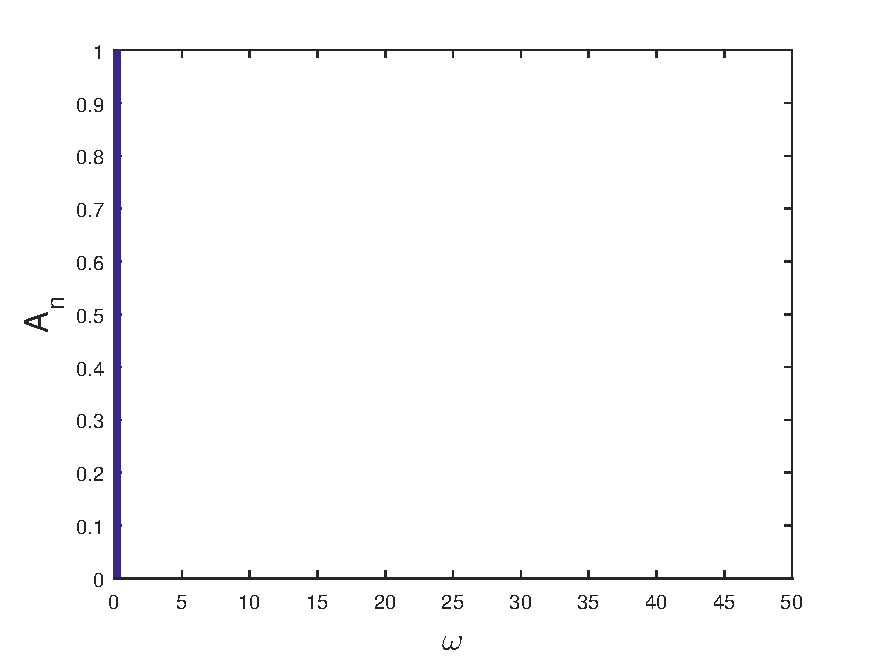
\includegraphics[width=0.49\textwidth]{kugel/Dkonstant/Rechteck4_2.pdf}
\caption{Titel??
\label{skript:Dirac2}}
\end{figure}

\section{Gibbsscher-Effekt} 
\rhead{Gibbsscher-Effekt}
Der gibbssche Effekt tritt immer dann auf, wenn eine Funktion Spr"unge aufweist. Bei der Original-Rechteckfunktion Abbildung \ref{skript:Gibborg} kann man einen solchen Sprung sehen. Beim rekonstruierten Rechtecksignal Abbildung \ref{skript:Gibbsre},  kann man erkennen dass der Sprung nicht ganz so steil ist und es vor und nach dem Sprung "uberschwingt. Dieselben Effekte sind in Abbildung \ref{skript:Gibbs1} und Abbildung \ref{skript:Gibbs2} auch auf der Kugeloberfl"ache zu erkennen. Mit n wird jeweils bezeichnet wie viele Koeffizienten für die Rekonstruktion der Funktionen verwendet wurden.


\begin{figure}
\begin{minipage}[hbt]{0.5\textwidth}
\centering
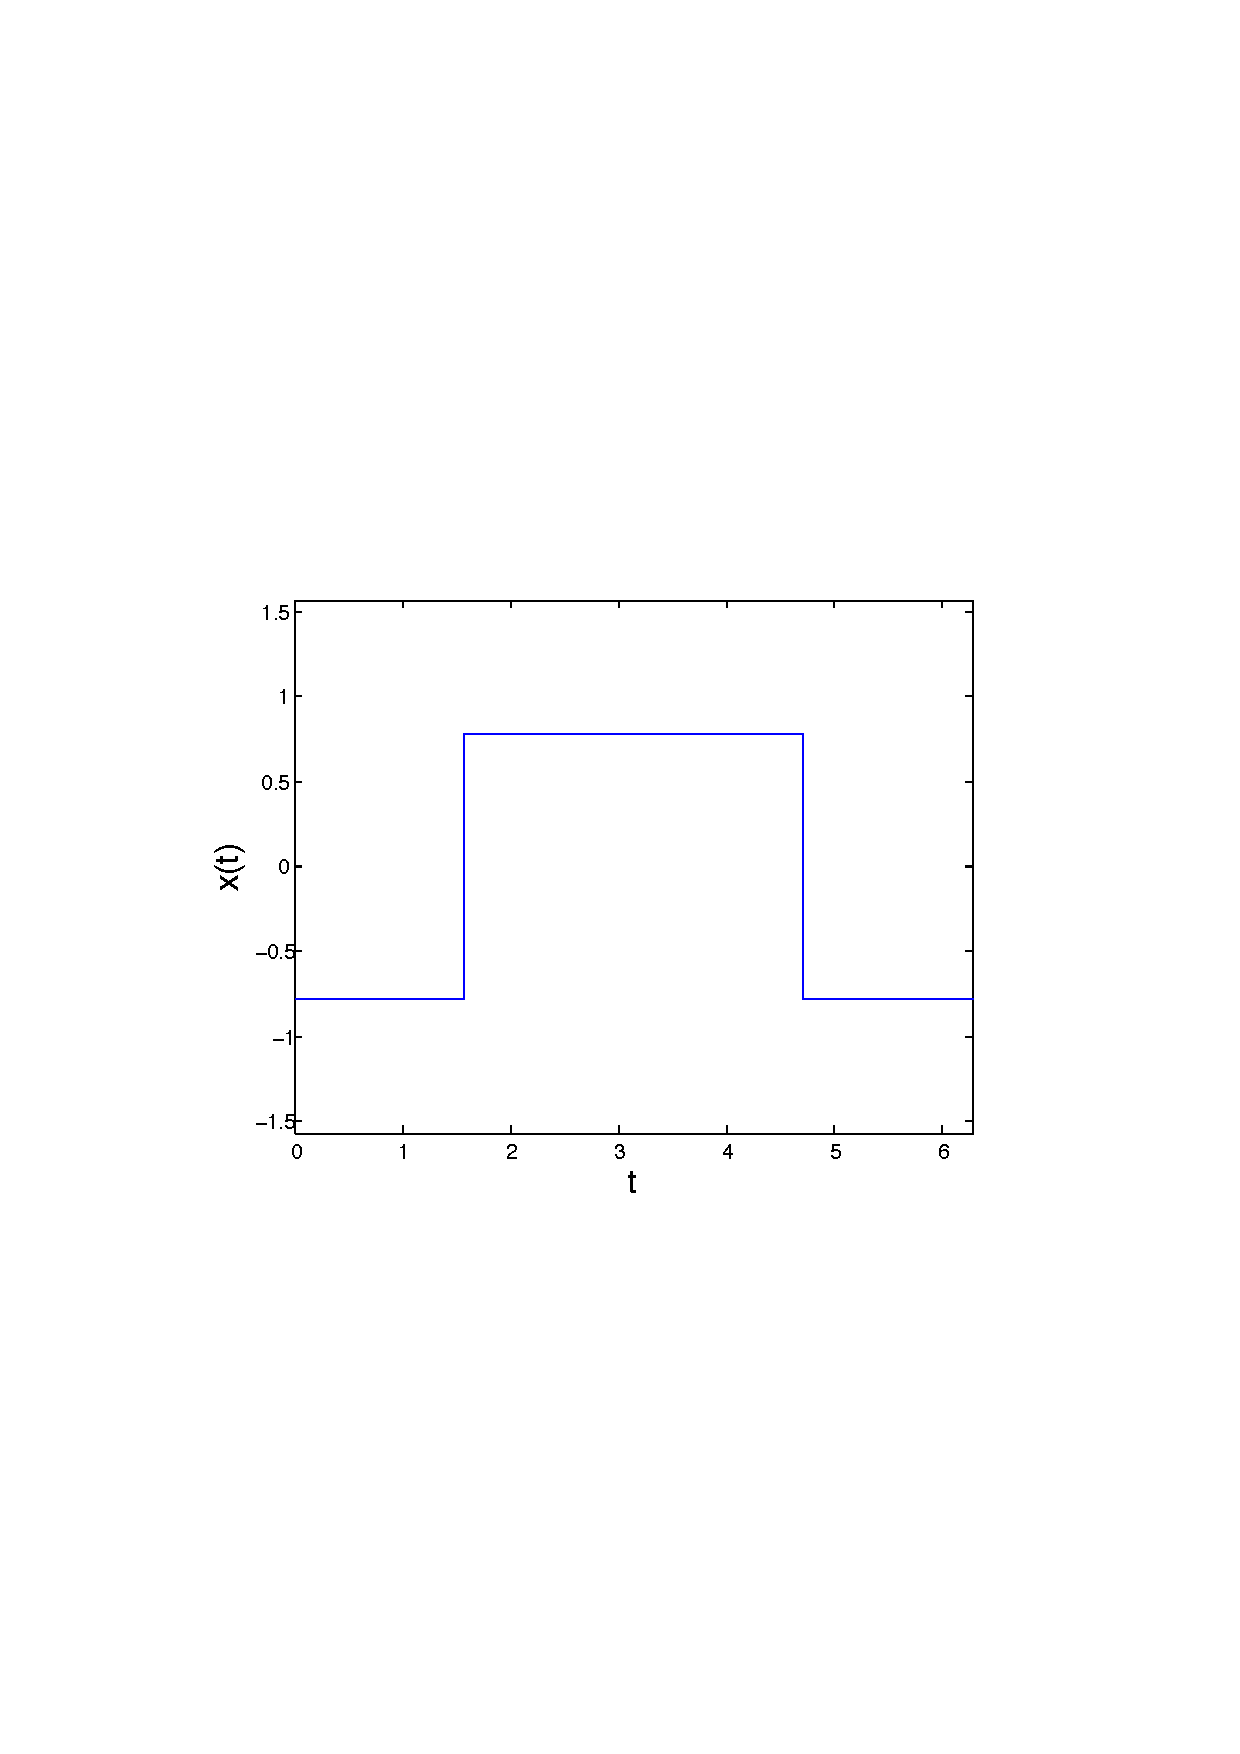
\includegraphics[width=1\textwidth]{kugel/Gibbs/Funktion.pdf}
\caption{Original-Rechteckfunktion}
\label{skript:Gibborg}
\end{minipage}
\hfill
\begin{minipage}[hbt]{0.5\textwidth}
\centering
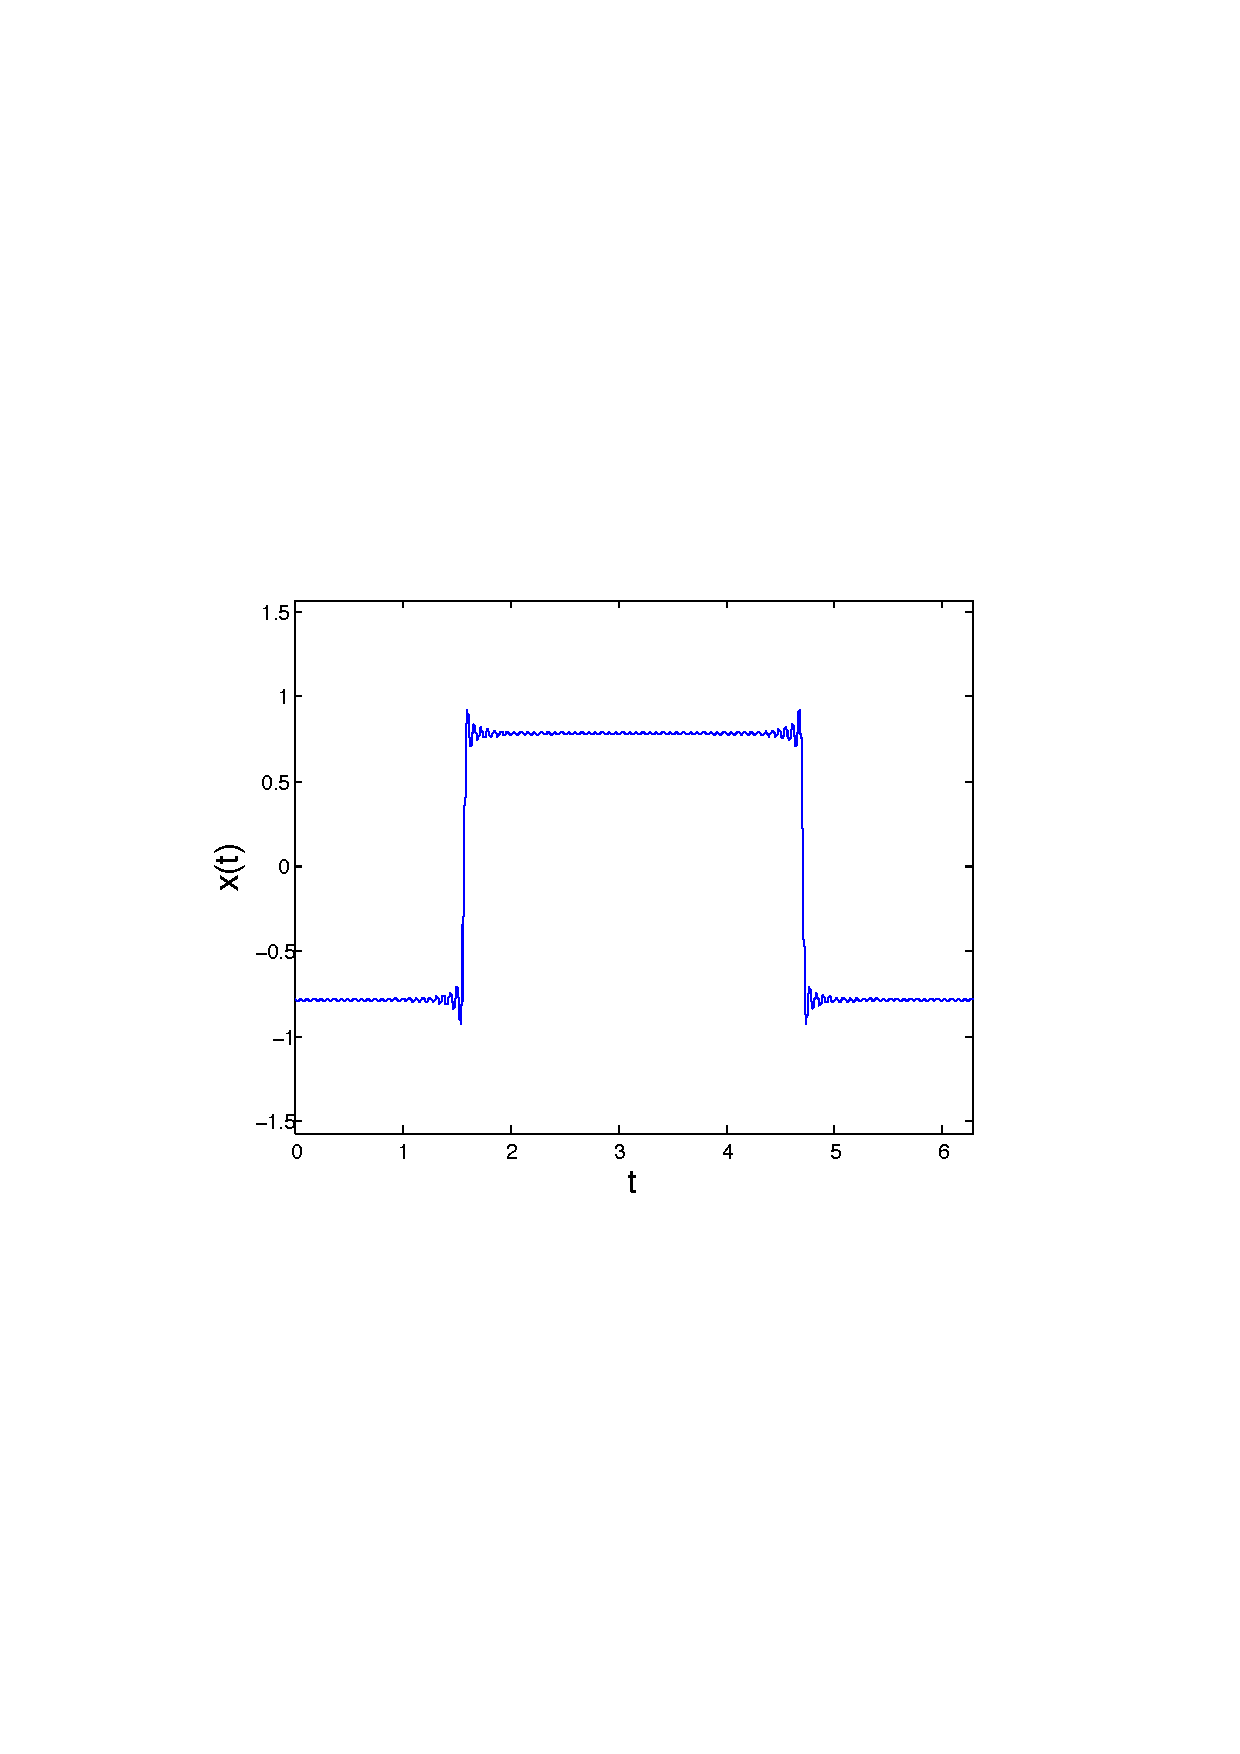
\includegraphics[width=1\textwidth]{kugel/Gibbs/Gibbs.pdf}
\caption{Rekonstruiertes Rechtecksignal}
\label{skript:Gibbsre}
\end{minipage}
\end{figure}

\begin{figure}% Gibbsscher-Effekt
\centering
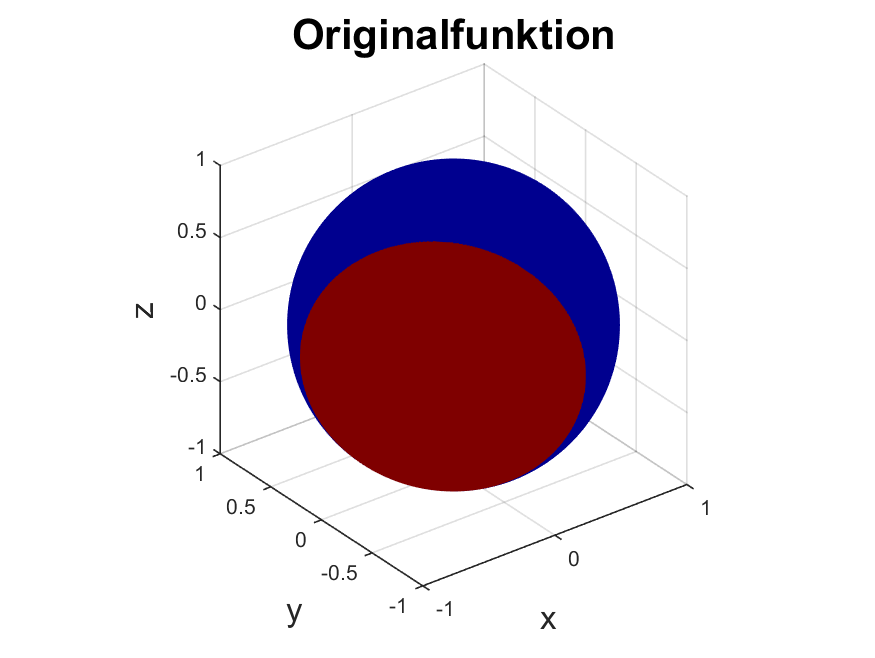
\includegraphics[width=0.4\textwidth]{kugel/Gibbs/GibbsOriginalFunktion.pdf}
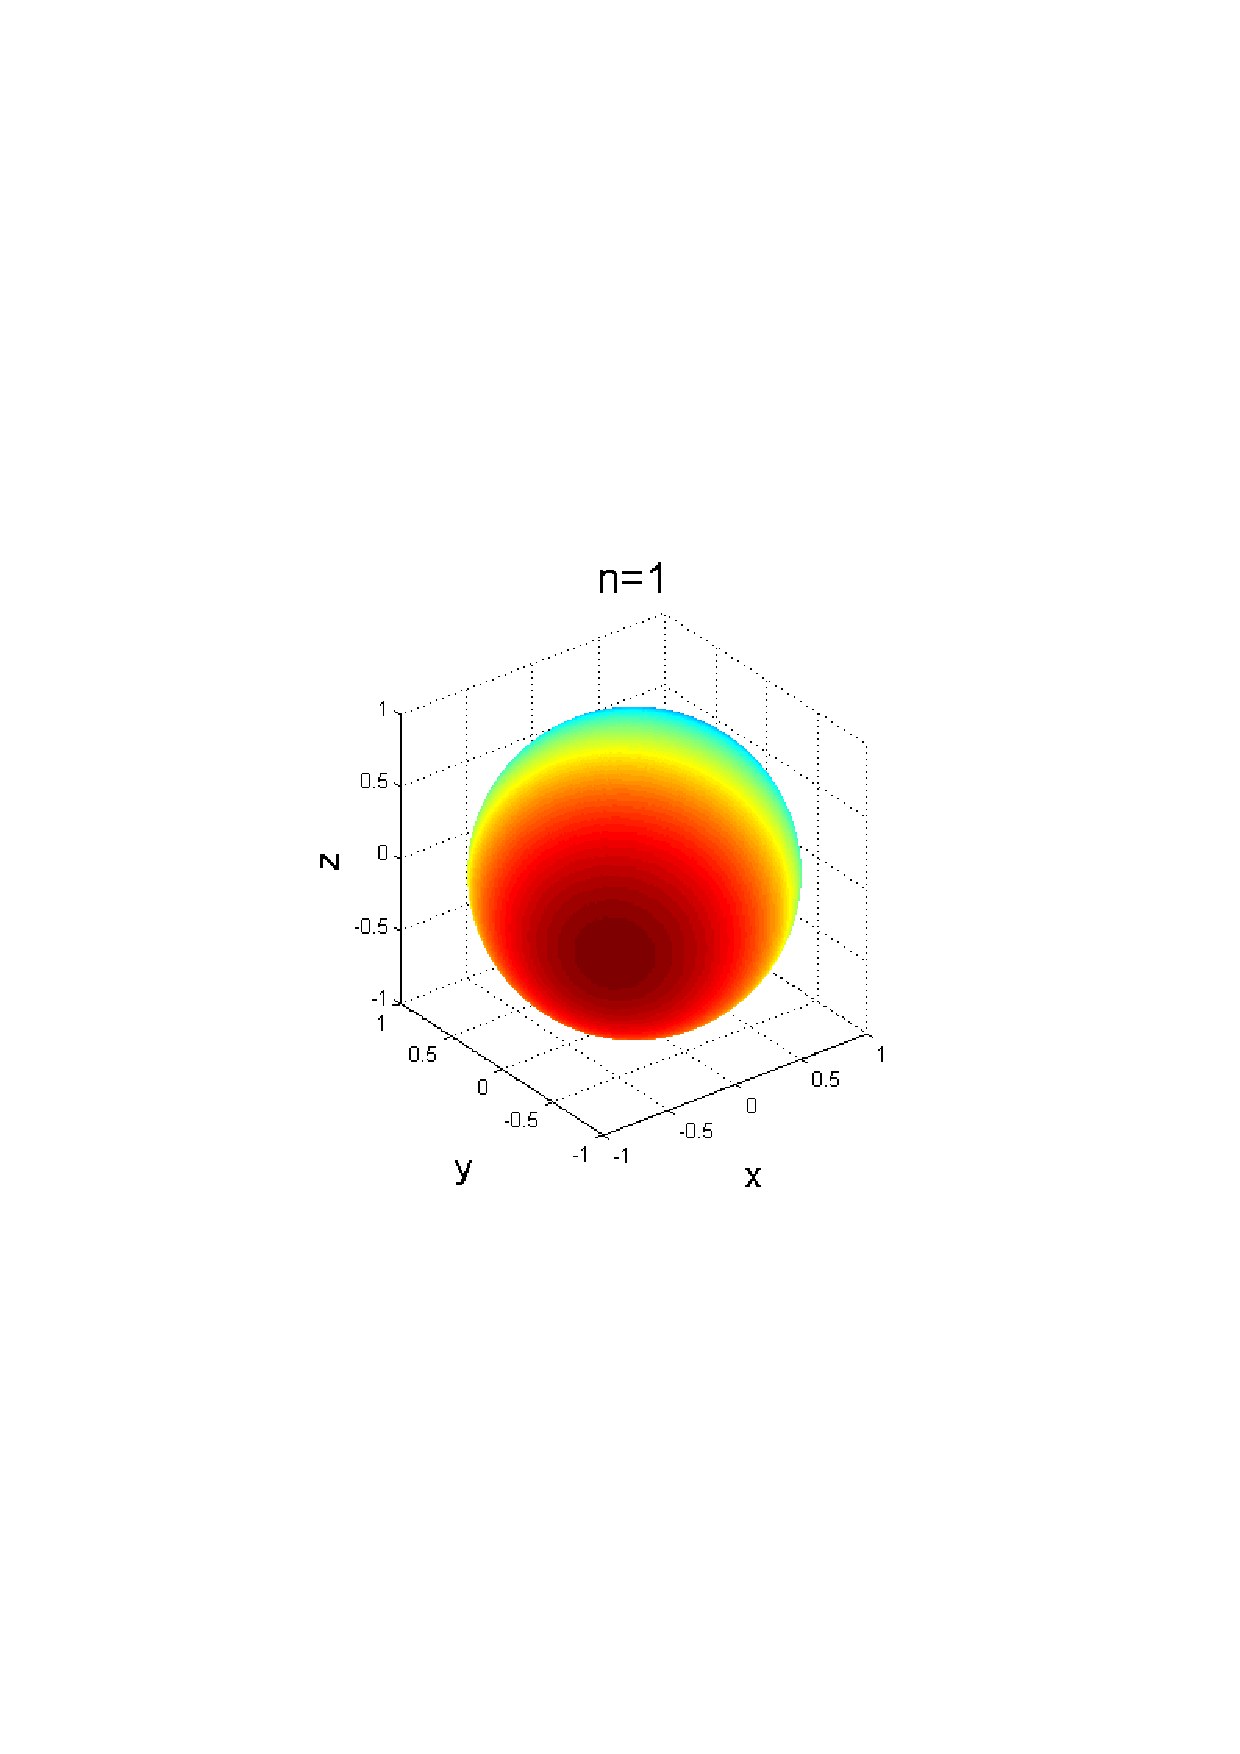
\includegraphics[width=0.4\textwidth]{kugel/Gibbs/GibbsN_1.pdf}
\includegraphics[width=0.4\textwidth]{kugel/Gibbs/GibbsN_2.pdf}
\includegraphics[width=0.4\textwidth]{kugel/Gibbs/GibbsN_3.pdf}
\includegraphics[width=0.4\textwidth]{kugel/Gibbs/GibbsN_4.pdf}
\includegraphics[width=0.4\textwidth]{kugel/Gibbs/GibbsN_5.pdf}
\caption{Gibbsscher-Effekt $n=1$ bis $n=5$
\label{skript:Gibbs1}}
\end{figure}

\begin{figure}% Gibbsscher-Effekt
\centering
\includegraphics[width=0.4\textwidth]{kugel/Gibbs/GibbsOriginalFunktion.pdf}
\includegraphics[width=0.4\textwidth]{kugel/Gibbs/GibbsN_10.pdf}
\includegraphics[width=0.4\textwidth]{kugel/Gibbs/GibbsN_15.pdf}
\includegraphics[width=0.4\textwidth]{kugel/Gibbs/GibbsN_20.pdf}
\includegraphics[width=0.4\textwidth]{kugel/Gibbs/GibbsN_25.pdf}
\includegraphics[width=0.4\textwidth]{kugel/Gibbs/GibbsN_30.pdf}
\caption{Gibbsscher-Effekt $n=10$ bis $n=30$
\label{skript:Gibbs2}}
\end{figure}

\section{Numerische Berechnung} 
\rhead{Numerische Berechnung}
Allf"allige Abweichungen in unseren Darstellungen sind auf die numerischen Berechnungen zur"uckzuf"uhren, da wir $d\vartheta$ und $d\varphi$ nicht beliebig klein w"ahlen konnten. Qualitativ sind jedoch alle Ergebnisse korrekt.

\printbibliography[heading=subbibliography]
\end{refsection}